%% LyX 2.1.3 created this file.  For more info, see http://www.lyx.org/.
%% Do not edit unless you really know what you are doing.
\documentclass[english]{article}
\usepackage{lmodern}
\usepackage[latin9]{inputenc}
\usepackage[a4paper]{geometry}
\geometry{verbose,tmargin=1in,bmargin=1in,lmargin=0.5in,rmargin=0.5in}
\usepackage{fancyhdr}
\pagestyle{fancy}
\setlength{\parskip}{\smallskipamount}
\setlength{\parindent}{0pt}
\usepackage{babel}
\usepackage{units}
\usepackage{amsmath}
\usepackage{amssymb}
\usepackage{graphicx}
\usepackage[unicode=true,
 bookmarks=true,bookmarksnumbered=false,bookmarksopen=false,
 breaklinks=true,pdfborder={0 0 0},backref=false,colorlinks=false]
 {hyperref}
\hypersetup{pdftitle={HSLU Zulassungsstudium Mathe Formelsammlung},
 pdfauthor={KevinHaeusler}}

\makeatletter

%%%%%%%%%%%%%%%%%%%%%%%%%%%%%% LyX specific LaTeX commands.
%% Because html converters don't know tabularnewline
\providecommand{\tabularnewline}{\\}

%%%%%%%%%%%%%%%%%%%%%%%%%%%%%% Textclass specific LaTeX commands.
\newenvironment{lyxlist}[1]
{\begin{list}{}
{\settowidth{\labelwidth}{#1}
 \setlength{\leftmargin}{\labelwidth}
 \addtolength{\leftmargin}{\labelsep}
 \renewcommand{\makelabel}[1]{##1\hfil}}}
{\end{list}}

%%%%%%%%%%%%%%%%%%%%%%%%%%%%%% User specified LaTeX commands.
\usepackage{tabularx}

\usepackage{pgf,tikz}
\usepackage{mathrsfs}
\usetikzlibrary{arrows}
\usepackage{multicol}
\usepackage{array}
\usepackage{pgfplots}
\usepackage{tocloft}
\addto\captionsenglish{% Replace "english" with the language you use
  \renewcommand{\contentsname}%
    {Inhaltsverzeichnis}%
}
\renewcommand{\cftsubsecfont}{\bfseries}
\usepgfplotslibrary{polar}
\usepgflibrary{shapes.geometric}
\usetikzlibrary{calc}
\pgfplotsset{my style polar/.append style={xticklabels={,, $\frac{\pi}{6}$, $\frac{\pi}{3}$, $\frac{\pi}{2}$, $\frac{2\pi}{3}$, $\frac{5\pi}{6}$, $\pi$, $\frac{7\pi}{6}$, $\frac{4\pi}{3}$, $\frac{3\pi}{2}$, $\frac{5\pi}{3}$,$\frac{11\pi}{6}$,}, thick }}
\setlength{\cftsubsecnumwidth}{3em}
\setlength{\cftbeforesubsecskip}{1em}

\makeatother

\begin{document}
\lhead{\textsf{\textbf{HSLU Zulassungsstudium Formelsammlung}}}
\rhead{\textsf{Kevin Haeusler}}
\title{\textsf{\textbf{HSLU Zulassungsstudium Formelsammlung}}}
\date{}


\maketitle
\begin{multicols}{2}

    \setlength{\parskip}{0.0in}

    \noindent \begin{flushleft}
        \tableofcontents{}
        \par\end{flushleft}

\end{multicols}

\setlength{\smallskip}\newpage{}



\begin{multicols}{2}
    \section{Grundlagen}
    \subsection{Zahlen und Logik}
    \subsubsection{Zahlenbereiche}

    \begin{tabularx}{0.5\textwidth} {
            | >{\raggedright\arraybackslash}c
            | >{\raggedright\arraybackslash}X
            | >{\raggedright\arraybackslash}c |}
        \hline
        \textbf{*}     & \textbf{Bedeutung}                    & \textbf{Beispiel}                            \\ \hline
        $\mathbb{N}$   & Ganze Positive Zahlen                 & 1;2;3;                                       \\ \hline
        $\mathbb{N}_0$ & Ganze Positive Zahlen mit 0           & 0;1;2;                                       \\ \hline
        $\mathbb{Z}$   & Ganze Zahlen                          & -1;0;1;                                      \\ \hline
        $\mathbb{Q}$   & Rationale Zahlen = Bruchzahlen        & $\frac{3}{7} $ $\frac{5}{9} $ $\frac{2}{3} $ \\ \hline
                       & Irrationale Zahlen = Nachkommastellen & 0.3281                                       \\ \hline
        $\mathbb{R}$   & Reele Zahlen = Q + Irrationale Zahlen & Alle                                         \\ \hline
    \end{tabularx}
    \subsubsection{Wachstum}
    Wachstumsfaktor: $q = 1 + \frac{p}{100}$

    Explizit: $B(t) = B(0) \cdot {\color{green}q}^t \quad \text{mit } {\color{green}q > 1}$ q = Prozent t = Zeit


    \subsubsection{Summe und Produkte}
    \textbf{Summezeichen:} \\
    Es sei:  n, k $\in$ Z und n $\geq$ k
    \[ \sum_{k=1}^{n} a_k = a_1 + a_2 + a_3 + \ldots + a_n \]
    k heisst Laufvariable, Laufindex oder Summationsvariable \\
    1 heisst Startwert oder untere Grenze \\
    n heisst Endwert oder obere Grenze \\
    $a_{k}$ ist die Funktion bezueglich der Laufvariable \\

    \textbf{Produktzeichen:}
    \[ \prod_{k=1}^{n} a_k = a_1 \cdot a_2 \cdot a_3 \cdot \ldots \cdot a_n\]
    k heisst Laufvariable oder Laufindex \\
    1 heisst Startwert oder untere Grenze \\
    n heisst Endwert oder obere Grenze \\
    $a_{k}$ ist die Funktion bezueglich der Laufvariable \\

    \subsubsection{Mengen Operationen}

    \begin{tabularx}{0.5\textwidth} {
            | >{\raggedright\arraybackslash}c
            | >{\raggedright\arraybackslash}X |}
        \hline
        \textbf{*}            & \textbf{Bedeutung}                                           \\ \hline
        $\varnothing$ oder {} & Leere Menge, enthält keine Elemente                          \\ \hline
        $x\in A$              & Beschreibt Element x ist in Menge A                          \\ \hline
        $x\notin A$           & Beschreibt Element x ist nicht in Menge A                    \\ \hline
        $A\subset B$          & A ist eine Teilmenge von B                                   \\ \hline
        $A\cap B$             & Schnittmenge von A und B                                     \\ \hline
        $A\cup B$             & Vereinigunsgsmenge von A und B                               \\ \hline
        $A\backslash B$       & Differenzbildung, Menge von A ohne B                         \\\hline
        $\bar{A}_B$           & $:= \{x \,|\, x \in B \enspace \wedge \enspace x \notin A\}$ \\\hline
    \end{tabularx}
    \\~\\
    \\~\\
    \\~\\

    \def\firstcircle{(0,0) circle (1cm)}
    \def\secondcircle{(0:1.2cm) circle (1cm)}

    \colorlet{circle edge}{blue!50}
    \colorlet{circle area}{blue!20}

    \tikzset{filled/.style={fill=circle area, draw=circle edge, thick},
        outline/.style={draw=circle edge, thick}}

    \setlength{\parskip}{5mm}
    % Set A and B
    \begin{tikzpicture}
        \begin{scope}
            \clip \firstcircle;
            \fill[filled] \secondcircle;
        \end{scope}
        \draw[outline] \firstcircle node {$A$};
        \draw[outline] \secondcircle node {$B$};
        \node[anchor=south] at (current bounding box.north) {$A \cap B$};
    \end{tikzpicture}
    \begin{tikzpicture}
        \draw[filled] \firstcircle node {$A$}
        \secondcircle node {$B$};
        \node[anchor=south] at (current bounding box.north) {$A \cup B$};
    \end{tikzpicture}

    % Set A but not B
    \begin{tikzpicture}
        \begin{scope}
            \clip \firstcircle;
            \draw[filled, even odd rule] \firstcircle node {$A$}
            \secondcircle;
        \end{scope}
        \draw[outline] \firstcircle
        \secondcircle node {$B$};
        \node[anchor=south] at (current bounding box.north) {$A\backslash  B$};
    \end{tikzpicture}
    \begin{tikzpicture}
        \draw[filled, even odd rule] \firstcircle node {$A$}
        \secondcircle node{$B$};
        \node[anchor=south] at (current bounding box.north) {$\overline{A \cap B}$};
    \end{tikzpicture}


    \begin{tabularx}{0.5\textwidth} {
            | >{\raggedright\arraybackslash}c
            | >{\raggedright\arraybackslash}X
            | >{\raggedright\arraybackslash}c |}
        \hline
        \textbf{*}            & \textbf{Bedeutung}                        & \textbf{Beispiel}             \\ \hline
        $|A|$                 & Kardinalität/Mächtigkeit beschreibt       & A = {1;2}                     \\
                              & Anzahl Elemente einer Menge               & |$|A|$ = 2                    \\ \hline
        $\land$               & Konkuktion/UND A $\land$ B = Wahr wenn    & A $\land$ B                   \\
                              & A und B beide Wahr sind                   & A, B = W                      \\ \hline
        $\lor$                & Disjunktion/ODER A $\lor$ B  = Wahr wenn  & {-1;0;1;}                     \\
                              & A oder B  jeweils Wahr ist                &                               \\ \hline
        $\neg$                & Negation A = Wahr$\neg$A = Falsch         & $\neg $A                      \\\hline
        $\implies$            & Implikation: Daraus folgt                 &                               \\ \hline
        $\Longleftrightarrow$ & äquivalenz A $\Longleftrightarrow$ B wenn &                               \\
                              & beide wahr oder falsch sind               &                               \\ \hline
        $\forall$             & für Alle                                  & $\forall$ $x \in \mathbb{N}$  \\ \hline
        $\exists$             & Es Existiert                              & $\exists $ $x \in \mathbb{N}$ \\ \hline
    \end{tabularx}

    \begin{tabular}{@{ }c@{ }@{ }c | c@{ }@{ }c@{ }@{ }c@{ }@{ }c@{ }@{ }c | c@{ }@{ }c@{ }@{ }c@{ }@{ }c@{ }@{ }c | c@{ }@{ }c | c@{ }@{ }c@{ }@{ }c@{ }@{ }c@{ }@{ }c@{ }@{ }c}
        A & B &  & A & $\land$            & B &  &  & A & $\lor$             & B &  & $\lnot$            & B &  & A & $\lor$             & $\lnot$ & B & \\
        \hline
        T & T &  & T & \textcolor{red}{T} & T &  &  & T & \textcolor{red}{T} & T &  & \textcolor{red}{F} & T &  & T & \textcolor{red}{T} & F       & T & \\
        T & F &  & T & \textcolor{red}{F} & F &  &  & T & \textcolor{red}{T} & F &  & \textcolor{red}{T} & F &  & T & \textcolor{red}{T} & T       & F & \\
        F & T &  & F & \textcolor{red}{F} & T &  &  & F & \textcolor{red}{T} & T &  & \textcolor{red}{F} & T &  & F & \textcolor{red}{F} & F       & T & \\
        F & F &  & F & \textcolor{red}{F} & F &  &  & F & \textcolor{red}{F} & F &  & \textcolor{red}{T} & F &  & F & \textcolor{red}{T} & T       & F & \\
    \end{tabular}

    \subsection{Prozentrechnen}
    \vspace{-4mm}
    \subsubsection{Definition}
    \vspace{-4mm}
    $\frac{\text{Prozentwert } W}{\text{Grundwert } G} = \frac{\text{Prozentzahl } p}{100} = \text{Prozentsatz } p\ \%$
    \subsubsection{Prozentwert berechnen}
    \vspace{-4mm}
    $(1) \text{ Prozentwert } W = \text{Prozentsatz } p\ \% \cdot \text{ Grundwert } G$\\
    $(2) \text{ Prozentwert } W = \frac{\text{Prozentzahl } p}{100} \cdot \text{ Grundwert } G$
    \subsubsection{Prozentsatz berechnen}
    \vspace{-4mm}
    $(1) \text{ Prozentzahl } p = \frac{\text{Prozentwert } W}{\text{Grundwert } G} \cdot 100$\\
    $(2) \text{ Prozentsatz } p\ \% = \frac{\text{Prozentwert } W}{\text{Grundwert } G} \cdot 100\ \%$
    \subsubsection{Grundwert berechnen }
    \vspace{-4mm}
    $(1) \text{ Grundwert } G = \text{Prozentwert } W:\text{Prozentsatz } p\ \%$\\
    $(2) \text{ Grundwert } G = \text{Prozentwert } W \cdot \frac{100}{\text{Prozentzahl } p}$
    \subsubsection{Prozentuale Veränderung}
    \vspace{-4mm}
    Eine prozentuale Veränderung ist die Veränderung einer Größe innerhalb eines bestimmten Zeitraums, ausgedrückt in Prozent.\\
    $\text{Anfangswert} \pm \text{Prozentuale Veränderung} = \text{Endwert}$
    \subsubsection{Prozentfaktor}
    \vspace{-4mm}
    $\text{Anfangswert } G \cdot \text{Prozentfaktor } q = \text{Endwert } G_{neu}$\\
    $\,q = \left(100\ \% \pm p\ \%\right)$\\
    $q = \left(1 \pm \frac{p}{100}\right)$

    Bei einer Zunahme ist der Prozentfaktor größer als 1 = Wachstumsfaktor\\.
    Bei einer Abnahme ist der Prozentfaktor kleiner als 1 = Abnahmefaktor.
    \subsubsection{Prozentuale Zunahme}
    \vspace{-4mm}
    $\text{Endwert } G_{neu+} = \text{Anfangswert } G \cdot \underbrace{\left(1 + \frac{p}{100}\right)}_{\text{Wachstumsfaktor}}$
    \subsubsection{Prozentuale Abnahme}
    \vspace{-4mm}
    $\text{Endwert } G_{neu-} = \text{Anfangswert } G \cdot \underbrace{\left(1 - \frac{p}{100}\right)}_{\text{Abnahmefaktor}}$


    \subsection{Aussagenlogik}
    \vspace{-4mm}
    \subsubsection{Definitionen}
    \vspace{-4mm}
    \textbf{Term:}  Ein Term ist eine sinnvolle Zusammensetzung von Zahlen,
    Variablen, Operationszeichen und Klammern.
    Ein Term hat keinen Wahrheitsgehalt, ist also weder wahr noch falsch. \\
    \textbf{Aussage:}
    Eine Aussage beschreibt durch Worte oder Zeichen einen Sachverhalt.
    Eine Aussage ist entweder wahr oder falsch. \\
    \textbf{Aussageform:}
    Jeder sprachliche oder zeichensymbolische Ausdruck mit wenigstens einer Variablen
    wenn er durch jede sinnvolle Belegung der Variablen jeweils eine Aussage wird.


    \section{Gleichungen}
    \vspace{-4mm}
    \subsection{Allgemein}
    \vspace{-4mm}
    \subsubsection{Definitionen}
    \vspace{-4mm}
    \textbf{Gleichungen lösen} \\
    Jede Zahl aus der Definitionsmenge, die beim Einsetzen für x zu einer wahren Aussage fuehrt, heisst loesung der Gleichung. \\
    \textbf{Grundmenge, Definitionsbereich} $\mathbb{D}$ \\
    Die Menge aus der die loesungen stammen duerfen. \\
    \textbf{loesungsvariable} \\
    Variable nach der aufgeloest wird. \\
    \textbf{Formvariablen, Parameter} \\
    Alle anderen Variablen. \\
    \textbf{loesungsmenge} \\
    Menge aller Elemente aus der Definitionsmenge, die zu einer wahren Aussage fuehren. \\
    \textbf{äquivalenz} \\
    Zwei Gleichungen sind äquivalent, wenn beim Ersetzen der Variablen durch die gleichen Elemente der "gemeinsamen" Definitonsmenge entweder beide in eine wahre oder falsche Aussage uebergehen.

    \subsubsection{Äquivalenzumformungen}
    \vspace{-4mm}
    Umformungen einer Gleichung, bei denen die Lösungsmenge gleich bleibt, heissen Äquivalenzumformungen.\\~\\
    \textbf{1. Termunformungen}\\
    $2x+5-3=0$ $\Longleftrightarrow$ $2x +2 = 0$ \\
    \textbf{2. Add./Sub.. mit der gleichen Zahl auf beiden Seiten} \\
    \textbf{3. Mult./Div. mit der gleichen Zahl auf beiden Seiten} \\
    Achtung: Ausser mit 0 \\
    \textbf{4. Beidseitige Add./Sub. mit dem gleichen Term} \\
    \textbf{5. Beidseitige Mult./Div. mit dem gleichen Term}

    \subsection{Lineare Gleichungen}
    \vspace{-4mm}
    \subsubsection{Definition}
    \vspace{-4mm}
    Eine Gleichung, die sich durch äquivalenzumformungen in die Form $ax + b = 0$ bringen lässt, heisst lineare Gleichung. Wir koennen lineare Gleichungen daran erkennen, dass die Variable nur in der 1. Potenz auftritt, also kein $x^2$, $x^3$\dots enthalten.

    \subsubsection{Lösen einer linearen Gleichung}
    \begin{enumerate}
        \item Gleichung nach $x$ auflösen
        \item loesungsmenge aufschreiben
    \end{enumerate}

    \subsection{Quadratische Gleichungen}
    \vspace{-4mm}
    \subsubsection{Definition}
    \vspace{-4mm}
    Gleichungen, die sich durch äquivalenzumformungen auf die Form $ax^2 + bx + c = 0 \quad (a, b, c \in \mathbb{R}; a \neq 0)$
    bringen lassen, heissen quadratische Gleichungen. Wir koennen quadratische Gleichungen daran erkennen, dass die Variable $x$ in der 2. Potenz $x^2$, aber in keiner hoeheren Potenz vorkommt. Es gibt 4 Arten/Formen von Quadratischen Gleichungen.
    \subsubsection{Lösen einer quadratischen Gleichung}
    \vspace{-4mm}
    \textbf{Lösung einer Reinquadratische Gleichung $ax^2 = 0$}
    Reinquadratische Gleichungen ohne Absolutglied besitzen als einzige loesung die Null.

    \begin{enumerate}
        \item Gleichung nach $x^2$ auflösen
        \item Wurzel ziehen
        \item loesungsmenge aufschreiben
    \end{enumerate}
    \textbf{Lösung einer Reinquadratische Gleichung mit Absolutglied $ax^2 + c = 0$}

    \begin{enumerate}
        \item Gleichung nach $x^2$ auflösen
        \item Wurzel ziehen
        \item loesungsmenge aufschreiben
    \end{enumerate}
    \textbf{Lösung einer Gemischtquadratische Gleichungen ohne Absolutglied $ax^2 + bx = 0$}

    \begin{enumerate}
        \item Quadratische Gleichung in Normalform bringen
        \item $x$ ausklammern
        \item  Faktoren gleich Null setzen
        \item Gleichung nach $x^2$ auflösen
        \item loesungsmenge aufschreiben
    \end{enumerate}

    \subsubsection{Mitternachtsformel}
    \vspace{-4mm}
    Gemischtquadratische Gleichungen $ax^2 + bx + c = 0$ mit Absolutglied lösen wir mit der Mitternachtsformel:
    \[x_{1/2} = \frac{-b \pm \sqrt{b^2 - 4ac}}{2a}\]\\~\\
    Fallunterscheidung:
    \[x_{1} = \dfrac{-b - \sqrt{b^2 - 4ac}}{2a}\]
    \[x_{2} = \dfrac{-b + \sqrt{b^2 - 4ac}}{2a}\]\\~\\

    \textbf{Übersicht}\\~\\
    \begin{tabularx}{0.5\textwidth} {
            | >{\raggedright\arraybackslash}X
            | >{\raggedright\arraybackslash}X
            | >{\raggedright\arraybackslash}X |}
        \hline
        \textbf{}                               & \textbf{Allgemeine Form}                       & \textbf{Normalform}                           \\ \hline
        Reinquadratisch ohne Absolutglied       & $2x^2 = 0$, $a = 2$, $b = 0$ und $c = 0$       & $x^2 = 0$, $a = 1$, $b = 0$ und $c = 0$       \\\hline
        Reinquadratisch mit Absolutglied        & $2x^2 -8 = 0$, $a = 2$, $b = 0$ und $c = -8$   & $x^2-4 = 0$, $a = 1$, $b = 0$ und $c = -4$    \\ \hline
        Gemischtquadrat- isch ohne Absolutglied & $2x^2-8x = 0$, $a = 2$, $b = -8$ und $c = 0$   & $x^2 -4x= 0$,  $a = 1$, $b = -4$ und $c = 0$  \\ \hline
        Gemischtquadrat- isch mit Absolutglied  & $2x^2-8x+6 = 0$, $a = 2$, $b = -8$ und $c = 6$ & $x^2-4x+3 = 0$, $a = 1$, $b = -4$ und $c = 3$ \\ \hline
    \end{tabularx}

    \textbf{Regeln}\\~\\
    Wenn das lineare Glied fehlt, gilt b = 0. \\
    Wenn das absolute Glied fehlt, gilt c = 0. \\
    Wenn das $x^2$ allein steht, gilt a = 0 (wegen $1 \cdot x^2 = x^2$).
    Wenn das x allein steht, gilt (wegen $1 \cdot x = x$).

    \textbf{Lösen einer Quadratischen Gleichung mit Mitternachtsformel}

    \begin{enumerate}
        \item Quadratische Gleichung in allgemeine Form bringen
        \item a, b und c aus der allgemeinen Form herauslesen
        \item  a, b und c in die Mitternachtsformel einsetzen
        \item loesung berechnen
        \item loesungsmenge aufschreiben
    \end{enumerate}

    \subsection{Bruchgleichung}
    \vspace{-4mm}
    \subsubsection{Definition}
    \vspace{-4mm}
    Eine Bruchgleichung ist eine Gleichung mit mindestens einem Bruchterm, in dem die Variable x im Nenner vorkommt.
    \subsubsection{Lösen einer Bruchgleichung}
    \vspace{-4mm}
    \begin{enumerate}
        \item Definitionsmenge bestimmen
        \item Gleichung nach $x$ auflösen
        \item Pruefen, ob der x-Wert in der Definitionsmenge ist
        \item loesungsmenge aufschreiben
    \end{enumerate}
    \subsubsection{Kehrwert}
    \vspace{-4mm}
    Wenn die Zähler der Brueche nur aus Zahlen bestehen, kann eine Kehrwertbildung sinnvoll sein.
    Den Kehrwert eines Bruchs erhält man durch Vertauschen von Zähler und Nenner.\\~\\
    \[\frac{{\colorbox{yellow}{$1$}}}{{\colorbox{orange}{$x$}}} = \frac{{\colorbox{yellow}{$2$}}}{{\colorbox{orange}{$x+1$}}} \Rightarrow  \frac{{\colorbox{orange}{$x$}}}{{\colorbox{yellow}{$1$}}} = \frac{{\colorbox{orange}{$x+1$}}}{{\colorbox{yellow}{$2$}}}\]


    \subsubsection{Multiplikation übers Kreuz}
    \vspace{-4mm}
    Wenn auf beiden Seiten der Gleichung jeweils ein Bruch steht, kann eine Multiplikation ueber Kreuz sinnvoll sein.
    \[\frac{{\colorbox{yellow}{$1$}}}{{\colorbox{orange}{$x$}}} = \frac{{\colorbox{orange}{$2$}}}{{\colorbox{yellow}{$x+1$}}} \Rightarrow {\colorbox{yellow}{$1$}} \cdot {\colorbox{yellow}{$x+1$}} = {\colorbox{orange}{$2$}} \cdot {\colorbox{orange}{$x$}}\]


    \subsection{Betragsgleichung}
    \vspace{-4mm}
    \subsubsection{Definition}
    \vspace{-4mm}
    Betragsgleichungen lassen sich durch Fallunterscheidung lösen.

    \subsubsection{Eigenschaften und Rechenregeln}
    \vspace{-4mm}
    für alle $a, b \in \mathbb{R}$ gilt: \\
    $|x| \geq 0$ Beträge sind nicht negativ! \\
    $|x| = 0 \Leftrightarrow x = 0$ \\
    $|a \cdot b| = |a| \cdot |b|$ daraus folgt: $|a^n| = |a|^n$ für $n \in \mathbb{N}$ \\
    $|\frac{a}{b}| = \frac{|a|}{|b|}$ für $b \neq 0$  daraus folgt: $|\frac{1}{a^n}| = \frac{1}{|a|^n}$ für $n \in \mathbb{N}$ $a \neq 0$ \\
    $ |a+b| \leq |a| + |b|$ Dreiecksungleichung

    \subsubsection{Lösen einer Betragsgleichung}
    \vspace{-4mm}

    \begin{equation*} |a| = \begin{cases} a &\text{für } a \geq 0 \\[5px] -a &\text{für } a < 0 \end{cases} \end{equation*}\\~\\
    Aus der Definition des Betrags ergeben sich folgende zwei Fälle: \\
    \begin{itemize}
        \item Wenn der Term im Betrag groesser oder gleich Null ist ($a \geq 0$), koennen wir den Term einfach ohne Betragsstriche schreiben ($|a| = a$)
        \item Wenn der Term im Betrag kleiner als Null ist ($a < 0$) , müssen wir die Vorzeichen des Terms umdrehen, um die Betragsstriche weglassen zu koennen ($|a| = -a$).
    \end{itemize}
    Die Lösungsmenge der einzelnen Fälle geben wir als Intervalle an. \\
    Die Lösungsmenge der Gleichung ist die Vereinigungsmenge der einzelnen loesungsmengen.\\~\\
    \textbf{Fallunterscheidung}
    \begin{enumerate}
        \item Betrag durch Fallunterscheidung auflösen
        \item loesungsmengen der einzelnen Fälle bestimmen
        \item loesungsmenge der Betragsgleichung bestimmen
    \end{enumerate}
    Aus der Definition des Betrags
    \begin{equation*} |a| = \begin{cases} a &\text{für } a \geq 0 \\[5px] -a &\text{für } a < 0 \end{cases} \end{equation*}\
    ergeben sich folgende zwei Fälle:
    Wenn der Term im Betrag groesser oder gleich Null ist ($a \geq 0$), koennen wir den Term einfach ohne Betragsstriche schreiben ($|a| = a$). \\
    Wenn der Term im Betrag kleiner als Null ist $a < 0$, müssen wir die Vorzeichen des Terms umdrehen, um die Betragsstriche weglassen zu koennen ($|a| = -a$).\\~\\
    \textbf{Quadrieren}
    \begin{enumerate}
        \item Betragsgleichung Quadrieren
        \item Gleichung lösen
    \end{enumerate}
    Durch Quadrieren verschwindet der Betrag, denn es gilt: $|a|^2 = a^2$.


    \subsection{Potenzgleichungen}
    \vspace{-4mm}
    \subsubsection{Definition}
    \vspace{-4mm}
    Eine Potenzgleichung ist eine Gleichung, die aus nur einer Potenz einer Variable und einer Konstanten besteht: $x^n = a$ \\~\\
    Die Vorgehensweise unterscheidet sich danach, wie der Exponent n aussieht:
    \begin{enumerate}
        \item Typ: $x^n = a$ mit n $\in \mathbb{N}$
        \item Typ: $x^{-n} = a$ mit n $\in \mathbb{N}$
        \item Typ: $x^{\frac{m}{n}} = a$ mit n $\in \mathbb{N}$ und mit $m \in \mathbb{Z}$
    \end{enumerate}
    Grundsätzlich lösen wir Potenzgleichungen durch Wurzelziehen. Das Problem ist, dass das Wurzelziehen im Allgemeinen keine äquivalenzumformung ist. Um zu verhindern, das loesungen verloren gehen, muss man bei geraden Exponenten Betragsstriche setzen:
    \begin{itemize}
        \item Wenn n gerade ist, gilt: $\sqrt[n]{x^n} = |x|$.
        \item Wenn n ungerade ist, gilt: $\sqrt[n]{x^n} = x$.
    \end{itemize}
    \subsubsection{Potenzgesetze}
    \vspace{-4mm}
    Multiplikation mit gleicher Basis = $x^a \cdot x^b = x^{a+b}$ \\
    Division mit gleicher Basis = $x^a : x^b = \frac{x^a}{x^b} = x^{a-b}$ \\
    Potenzen potenzieren = $\left(x^a\right)^b = x^{a \cdot b}$ \\
    Multiplikation mit gleichem Exponenten = $a^n \cdot b^n = \left(a \cdot b\right)^n$ \\
    Division mit gleichem Exponenten = $a^n : b^n = \frac{a^n}{b^n} = \left(\frac{a}{b}\right)^n$ \\
    Negative Exponenten: $x^{-n} = \frac{1}{x^n}$ \\
    Brüche als Exponenten: $x^{\frac{1}{n}} = \sqrt[n]{x}$ $x^{\frac{m}{n}} = \sqrt[n]{x^m}$ \\

    \subsubsection{Lösen einer Potenzgleichung}
    \vspace{-4mm}
    \textbf{Typ 1:  $x^n = a$ ($n \in \mathbb{N}$;$a \in \mathbb{R}$)} \\
    Vorgehensweise: n-te Wurzel ziehen\\
    Mögliche Lösungen \\
    \begin{tabularx}{0.5\textwidth} {
            | >{\raggedright\arraybackslash}c
            | >{\raggedright\arraybackslash}X
            | >{\raggedright\arraybackslash}X |}
        \hline
        \textbf{} & \textbf{n ist gerade}                        & \textbf{n ist ungerade}           \\ \hline
        $a > 0$   & $\mathbb{L} = \{-\sqrt[n]{a};+\sqrt[n]{a}\}$ & $\mathbb{L} = \{+\sqrt[n]{a}\}$   \\ \hline
        $a = 0$   & $\mathbb{L} = \{0\}$                         & $\mathbb{L} = \{0\}$              \\ \hline
        $a < 0$   & $\mathbb{L} = \{\}$                          & $\mathbb{L} = \{-\sqrt[n]{|a|}\}$ \\ \hline
    \end{tabularx}

    \textbf{Typ 2:} $x^{-n} = a$\\
    Vorgehensweise: Umformung der Gleichung zu Typ 1 (falls $a \neq 0$)\\
    Mögliche Lösungen
    \begin{itemize}
        \item  $a = 0$ Es gibt keine loesung $\mathbb{L} = \{\}$.
        \item  $a \neq 0$ Die Gleichung $x^{-n} = a$ ist äquivalent zu $x^n = \frac{1}{a}$.
    \end{itemize}
    \textbf{Typ 3:} $m \in \mathbb{Z}$ \\
    Vorgehensweise: Potenzieren mit n\\
    Ist der Exponent $\frac{m}{n}$ keine ganze Zahl, so sind die Gleichungen in $\mathbb{R}^{-}$ nicht definiert. In $\mathbb{R}_{0}^{+}$ sind die Gleichungen $x^{\frac{m}{n}} = a$ und $\sqrt[n]{x^m} = a$ äquivalent.\\

    \subsection{Wurzelgleichung}
    \vspace{-4mm}
    Eine Wurzelgleichung ist eine Gleichung, bei der die Variable (auch) unter einer Wurzel vorkommt.
    \subsubsection{Wurzel Gesetze}
    \vspace{-4mm}
    Wurzel Addieren = $a{\color{green}\sqrt[n]{x}} + b{\color{green}\sqrt[n]{x}} = (a + b){\color{green}\sqrt[n]{x}}$ \\
    Wurzel Subtrahieren = $a {\color{green}\sqrt[n]{x}} - b{\color{green}\sqrt[n]{x}} = (a - b){\color{green}\sqrt[n]{x}}$ \\
    Wurzel Multiplizieren = $\sqrt[{\color{green}n}]{a} \cdot \sqrt[{\color{green}n}]{b} = \sqrt[{\color{green}n}]{a \cdot b}$ \\
    Wurzel Potenzieren = $(\sqrt[n]{a})^m = \sqrt[n]{a^m}$ \\
    Wurzel Radizieren = $\sqrt[m]{\sqrt[n]{a}} = \sqrt[m \cdot n]{a}$ \\
    Wurzel in Potenz umformen = $\sqrt[n]{a} = a^{\frac{1}{n}}$ oder $\sqrt[n]{a^m} = a^{\frac{m}{n}}$ \\
    Wurzel Quadrieren: $\sqrt[]{a^2} = {(\sqrt[]{a})}^2 = a$ für $a \geq 0$ \\
    Folgerung: $\sqrt[]{a^2} = |a|$

    \subsubsection{Wurzelgleichung lösen}
    \vspace{-4mm}

    \begin{enumerate}
        \item Wurzeln beseitigen
              \begin{enumerate}
                  \item Wurzel isolieren
                  \item Potenzieren
              \end{enumerate}
        \item Algebraische Gleichung lösen
        \item Probe Machen
        \item Lösungsmenge aufschreiben
    \end{enumerate}
    \textbf{Erklärung:} \\
    Wurzel isolieren = Gleichung so umformen, dass die Wurzel allein auf einer Seite steht. \\~\\
    Um die Wurzel $\sqrt[n]{x}$ zu beseitigen, müssen wir sie mit dem Wurzelexponenten potenzieren. Das Potenzieren mit 2, um eine Quadratwurzel $\sqrt{x}$ zu beseitigen, heisst auch "Quadrieren". \\~\\
    Ziel des Potenzierens aus Schritt 1.2 ist es, die Wurzelgleichung in eine algebraische Gleichung (z.B. lineare Gleichung, quadratische Gleichung oder kubische Gleichung) zu ueberfuehren. Diese Gleichung koennen wir dann mit den bekannten Methoden lösen. \\~\\
    Das Potenzieren aus Schritt 1.2 ist i. Allg. keine äquivalenzumformung: Durch das Potenzieren koennen loesungen (sog. Scheinloesungen) hinzukommen, es gehen aber keine verloren.
    Um Scheinloesungen auszusortieren, machen wir die Probe, d.h., wir setzen die moeglichen loesungen in die Ausgangsgleichung ein. Nur die loesungen, die zu einer wahren Aussage fuehren, gehoeren auch wirklich zur loesung der Wurzelgleichung.


    \subsection{Exponential- und Logarithmusgleichungen}
    \vspace{-4mm}
    \subsubsection{Definition}
    \vspace{-4mm}
    Eine Exponentialgleichung ist eine Gleichung, in der die Variable im Exponenten einer Potenz steht. \\
    Eine Logarithmusgleichung ist eine Gleichung, in der die Variable im Numerus des Logarithmus steht.
    \[a^{f(x)} = b^{g(x)} \quad \Rightarrow \quad f(x) \cdot \log a = g(x) \cdot \log b\]

    Logarithmen mit der Basis e (der eulerschen Zahl) heissen natuerliche Logarithmen.
    \begin{equation*}
        e = \lim\limits_{n\rightarrow\infty}{\left(1+\frac{1}{n}\right)^n}.
    \end{equation*}
    \noindent
    $\exp{x} = e^x$ und $\ln{x}$ sind Kehrwertfunktionen
    \begin{equation*}
        e^{\ln{x}} = x \text{ and } \ln{e^x} = x.
    \end{equation*}

    \noindent
    Exponentenregeln für Exponentengleichung
    \begin{equation*}
        e^xe^y = e^{x+y} \text{, } \frac{e^x}{e^y}=e^{x-y} \text{, and } \left(e^x\right)^k=e^{xk}.
    \end{equation*}

    \noindent
    Exponentenregeln für Logarithmengleichung
    \begin{equation*}
        \ln{x}+\ln{y} = \ln{xy} \text{, } \ln{x}-\ln{y} = \ln{\left(\frac{x}{y}\right)} \text{, and } \ln{\left(a^b\right)} = b\ln{a}.
    \end{equation*}

    \noindent
    Wir koennen auch einen Logarithmus jeder Basis schreiben, indem wir natürliche Logarithmen verwenden:
    \begin{equation*}
        \log_{b}{a} = \frac{\ln{a}}{\ln{b}}.
    \end{equation*}

    \textbf{Lösung mithilfe der Definition des Logarithmus}\\
    Eine Lösung mithilfe der Definition des Logarithmus ist nur dann möglich, wenn es gelingt, die Terme auf beiden Seiten der Gleichung so umzuformen, dass sich auf der einen Seite ein Logarithmus und auf der anderen Seite eine Konstante ergeben.

    \textbf{Definitionsmenge einer Logarithmusgleichung }\\
    Da $\log_{b}x = a$  nur für $x > 0$ definiert ist, kann die Definitionsmenge eingeschränkt sein.
    In der Praxis bedeutet das, dass wir stets die Probe machen sollten, d.h. überprüfen, ob die berechneten Lösungen eingesetzt in die gegebene Gleichung zu einer wahren Aussage führen.
    \subsubsection{Logarithmengesetze}
    \vspace{-4mm}
    Produktregel: $\log_b(P \cdot Q) = \log_b P + \log_b Q$ \\
    Quotientregel: $\log_b\left(\frac{P}{Q}\right) = \log_b P - \log_b Q$ \\
    Potenzregel 1: $\log_b P^n = n \cdot \log_b P$ \\
    Potenzregel 2: $\log_b \sqrt[n]{P} = \frac{\log_b P}{n}$ \\
    Basiswechsel: $\log_a P = \frac{\log_b P}{\log_b a}$




    \subsection{Lineare Gleichungssysteme}
    \vspace{-4mm}
    \subsubsection{Definition}
    \vspace{-4mm}
    Mehrere lineare Gleichungen, die alle zusammen gelten sollen, bilden ein lineares Gleichungssystem.\\
    \subsubsection{Gleichsetzungsverfahren}
    \vspace{-4mm}
    \begin{enumerate}
        \item Gleichungen nach der gleichen Variable auflösen
        \item Gleichungen gleichsetzen
        \item Gleichung nach der enthaltenen Variable auflösen
        \item Berechneten Wert in eine der umgeformten Gleichungen aus Schritt 1 einsetzen und zweiten Wert berechnen
        \item loesungsmenge aufschreiben
    \end{enumerate}

    \subsubsection{Einsetzungsverfahren}
    \vspace{-4mm}
    \begin{enumerate}
        \item     Eine Gleichung nach einer Variable auflösen
        \item     Berechneten Term für diese Variable in die andere Gleichung einsetzen
        \item     Gleichung nach der enthaltenen Variable auflösen
        \item     Berechneten Wert in die umgeformte Gleichung aus Schritt 1 einsetzen und zweiten Wert berechnen
        \item     loesungsmenge aufschreiben
    \end{enumerate}

    \subsubsection{Additionsverfahren}
    \vspace{-4mm}
    \begin{enumerate}
        \item     Gleichungen so umformen, dass die Koeffizienten einer Variablen Gegenzahlen werden
        \item     Gleichungen addieren
        \item     Gleichung nach der enthaltenen Variable auflösen
        \item     Berechneten Wert in eine der urspruenglichen Gleichungen einsetzen und zweiten Wert berechnen
        \item     loesungsmenge aufschreiben
    \end{enumerate}
    Damit die Koeffizienten der Variablen Gegenzahlen werden, bilden wir das kleinste gemeinsame Vielfache (kgV) der Koeffizienten und formen die Gleichungen anschliessend entsprechend um.

    \subsection{Ungleichungen}
    \vspace{-4mm}
    \subsubsection{Definition}
    \vspace{-4mm}
    Eine Ungleichung ist ein mathematischer Ausdruck, der aus zwei Termen besteht, die durch eines der Vergleichszeichen < (Kleinerzeichen), $\leq$ (Kleinergleichzeichen),
    > (Grösserzeichen) oder $\geq$ (Grössergleichzeichen) verbunden sind.

    \subsubsection{Rechenregeln}
    \vspace{-4mm}
    $ a < b \quad \Longleftrightarrow \quad b > a$\\
    $a \leq b \quad \Rightarrow \quad a+c \leq b+c$\\
    $a \leq b \quad\text{und}\quad c \leq d \quad \Rightarrow \quad a+c \leq b+d$\\
    $a < b \quad\text{und}\quad c \leq d \quad \Rightarrow \quad a+c < b+d$\\
    $a \leq b \quad\text{und}\quad c \geq 0 \quad \Rightarrow \quad ac \leq bc$\\
    $a \leq b \quad\text{und}\quad c \leq 0 \quad \Rightarrow \quad ac \geq bc$
    $a \leq b \quad \Rightarrow \quad \frac{1}{a} \geq \frac{1}{b}$ \\
    \subsubsection{Lineare Ungleichungen}
    \vspace{-4mm}
    \begin{enumerate}
        \item Ungleichung nach x auflösen
        \item Lösungsmenge aufschreiben
    \end{enumerate}
    \begin{itemize}
        \item Terme auf beiden Seiten der Ungleichung zusammenfassen
        \item Denselben Term auf beiden Seiten der Ungleichung addieren/subtrahieren
        \item Beide Seiten der Ungleichung mit derselben positiven* Zahl multiplizieren
        \item Beide Seiten der Ungleichung durch dieselbe positive* Zahl dividieren
    \end{itemize}
    * Bei der Multiplikation bzw. Division mit einer negativen Zahl müssen wir das Ungleichungszeichen umdrehen.
    \subsubsection{Quadratische Ungleichungen}
    \vspace{-4mm}
    Eine Ungleichung, die sich durch Äquivalenzumformungen in eine der Formen bringen lässt, heisst quadratische Ungleichung.\\
    $ax^2 + bx + c < 0$\\
    $ax^2 + bx + c > 0$\\
    $ax^2 + bx + c \leq 0$\\
    $ax^2 + bx + c \geq 0$\\
    \begin{enumerate}
        \item Quadratische Gleichung lösen
        \item Potenzielle Lösungsintervalle aufstellen
        \item Überprüfen, welche Lösungsintervalle zur Lösung gehören
    \end{enumerate}
    Eine quadratische Gleichung besitzt entweder keine Lösung, eine Lösung oder zwei Lösungen.
    \subsubsection{Bruchungleichungen}
    \vspace{-4mm}
    Bei Bruchungleichungen gibt es 2 Fälle:

    \textbf{Rechte Seite der Ungleichung $\neq$ 0}
    \begin{enumerate}
        \item Bruch durch Fallunterscheidung auflösen
        \item Lösungsmengen der einzelnen Fälle bestimmen (Intervalle)
        \item Lösungsmenge der Bruchungleichung bestimmen
    \end{enumerate}
    \begin{equation*} \frac{\text{Z}}{\text{N}} > c = \begin{cases} \frac{\text{Z}}{\text{N}} \cdot \text{N} > c \cdot \text{N} &\text{für } \text{N} > 0 \\[5px] \frac{\text{Z}}{\text{N}} \cdot \text{N} < c \cdot \text{N} &\text{für } \text{N} < 0 \end{cases} \end{equation*}
    Das Auflösen des Bruchs geschieht durch Multiplikation der Ungleichung mit dem Nenner des Bruchs. Dabei müssen wir jedoch eine Fallunterscheidung vornehmen. Ist der Nenner nämlich negativ, dreht sich das Ungleichheitszeichen um.
    \begin{equation*} \frac{\text{Z}}{\text{N}} > c = \begin{cases} \text{Z} > c \cdot \text{N} &\text{für } \text{N} > 0 \\[5px] \text{Z} < c \cdot \text{N} &\text{für } \text{N} < 0 \end{cases} \end{equation*}
    Die Lösungsmenge der Ungleichung ist die Vereinigungsmenge der einzelnen Lösungsmengen.


    \textbf{Rechte Seite der Ungleichung = 0}
    \begin{enumerate}
        \item Definitionsbereich bestimmen
        \item Nullstellen berechnen
        \item Intervallweise Betrachtung
    \end{enumerate}

    \newpage


    \section{Funktionen}
    \vspace{-4mm}
    \subsection{Lineare Funktionen}
    \vspace{-4mm}
    \subsubsection{Definiton}
    \vspace{-4mm}
    Eine Funktion $f$ mit der Funktionsgleichung $f(x) = mx + n$ heisst lineare Funktion. \\
    Wegen $y = f(x)$ koennen wir statt $f(x) = mx + n$ auch $y = mx + n$ schreiben:
    \begin{itemize}
        \item $y$: Abhängige Variable, y-Wert, Funktionswert
        \item $m$: Steigung
        \item  $x$: Unabhängige Variable, x-Wert, (Funktions-)Argument
        \item $n$ : y-Achsenabschnitt
    \end{itemize}
    \subsubsection{Achsenabschnitte verändern}
    \vspace{-4mm}
    Wenn wir den y-Achsenabschnitt n in $f(x) = mx + n$ verändern, passiert Folgendes:
    \begin{itemize}
        \item Gilt $n > 0$, ist die Gerade nach oben verschoben.
        \item Gilt $n < 0$ , ist die Gerade nach unten verschoben.
    \end{itemize}

    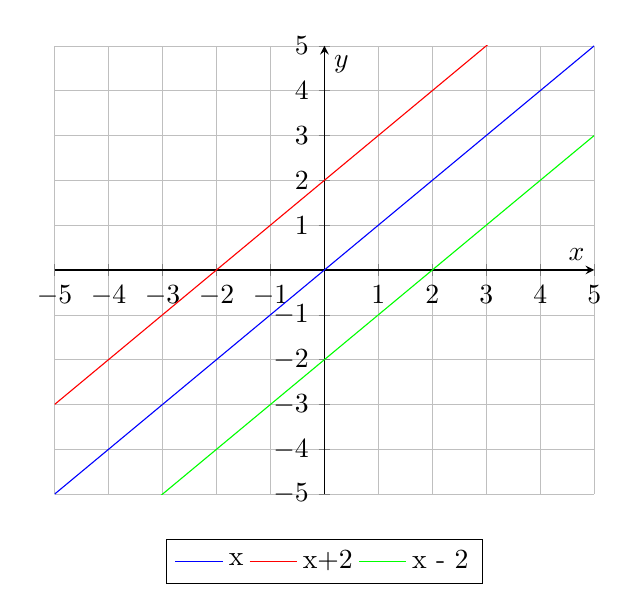
\begin{tikzpicture}%[scale=1.0]
        \begin{axis}[
                xlabel=$x$,
                ylabel=$y$,
                xmax=5,
                xmin=-5,
                ymax=5,
                ymin=-5,
                axis x line=middle,
                axis y line=middle,
                legend style={at={(0.5,-0.1)},
                        anchor=north,legend columns=-1},
                grid=major,
                grid style={line width=.1pt, draw=gray!10},
                major grid style={line width=.2pt,draw=gray!50},
                xtick={-5,-4,-3,-2,-1,0,1,2,3,4,5},
                ytick={-5,-4,-3,-2,-1,0,1,2,3,4,5}
            ]
            \addplot [blue] {x};
            \addlegendentry {x};
            \addplot [red] {x+2};
            \addlegendentry {x+2};
            \addplot [green] {x-2};
            \addlegendentry {x - 2};
        \end{axis}
    \end{tikzpicture}\\~\\
    Wenn wir die Steigungt m in $f(x) = mx + n$ verändern, passiert Folgendes:
    \begin{itemize}
        \item Gilt $m > 0$, steigt die Gerade.
        \item Gilt $m < 0$ , fällt die Gerade.
    \end{itemize}
    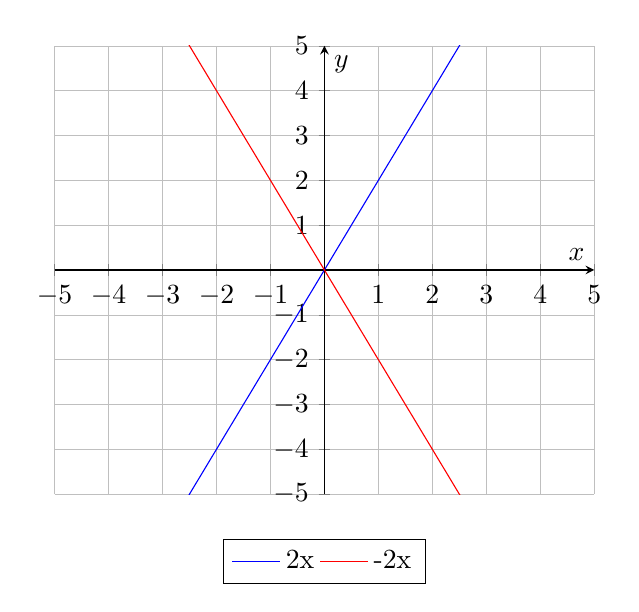
\begin{tikzpicture}%[scale=1.0]
        \begin{axis}[
                xlabel=$x$,
                ylabel=$y$,
                xmax=5,
                xmin=-5,
                ymax=5,
                ymin=-5,
                axis x line=middle,
                axis y line=middle,
                legend style={at={(0.5,-0.1)},
                        anchor=north,legend columns=-1},
                grid=major,
                grid style={line width=.1pt, draw=gray!10},
                major grid style={line width=.2pt,draw=gray!50},
                xtick={-5,-4,-3,-2,-1,0,1,2,3,4,5},
                ytick={-5,-4,-3,-2,-1,0,1,2,3,4,5}
            ]
            \addplot [blue] {x*2};
            \addlegendentry {2x};
            \addplot [red] {x*-2};
            \addlegendentry {-2x};
        \end{axis}
    \end{tikzpicture}

    \subsubsection{Nullstelle berechnen}
    \vspace{-4mm}

    Berechne die Nullstelle der linearen Funktion  $y = 3x + 3$. \\
    Wir setzen die Funktion gleich Null, d.h. wir setzen für den y Wert 0 ein: ${\color{red}{0}} = 3x + 3$ \\
    Jetzt müssen wir die Gleichung nach x auflösen, um die gesuchte Nullstelle zu finden.
    \subsubsection{Steigung berechnen}
    Wir lesen zwei beliebige Punkte ab:
    \[P_0({\color{blue}0}|{\color{red}1}) \text{ und } P_1({\color{blue}4}|{\color{red}3})\]
    und setzen sie in die Steigungsformel ein:
    \begin{align*} m &= \frac{y_1 - y_0}{x_1 - x_0} \\[5px] &= \frac{{\color{red}3} - ({\color{red}1})}{{\color{blue}4} - {\color{blue}0}}\\[5px] &= \frac{2}{4} \\[5px] &= \frac{1}{2} \end{align*}
    \subsubsection{Schnittpunkt berechnen}
    \vspace{-4mm}

    Ein Schnittpunkt existiert nur, wenn die beiden gegebenen Geraden eine unterschiedliche Steigung besitzen.
    \[g\colon~y = {\color{red}2}x + 1\]
    \[h\colon~y = {\color{red}2}x + 3\]
    Die Geraden besitzen dieselbe Steigung das heisst: \textbf{Es existiert kein Schnittpunkt}.\\
    Ansonsten gilt:
    \begin{enumerate}
        \item Funktionsgleichungen gleichsetzen
        \item Gleichung nach x auflösen
        \item x in eine der beiden Funktionsgleichungen einsetzen, um y zu berechnen
        \item Ergebnis aufschreiben
    \end{enumerate}

    \subsubsection{Umkehrfunktion bilden}
    \vspace{-4mm}

    \begin{enumerate}
        \item Funktionsgleichung nach x auflösen
        \item x und y vertauschen
    \end{enumerate}

    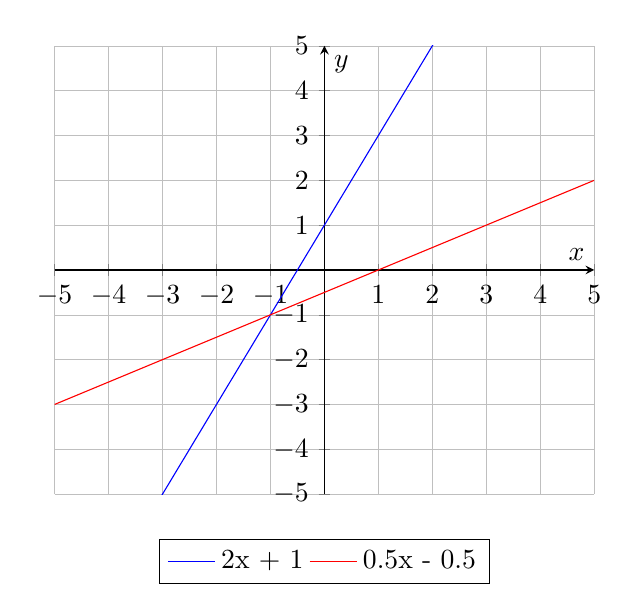
\begin{tikzpicture}%[scale=1.0]
        \begin{axis}[
                xlabel=$x$,
                ylabel=$y$,
                xmax=5,
                xmin=-5,
                ymax=5,
                ymin=-5,
                axis x line=middle,
                axis y line=middle,
                legend style={at={(0.5,-0.1)},
                        anchor=north,legend columns=-1},
                grid=major,
                grid style={line width=.1pt, draw=gray!10},
                major grid style={line width=.2pt,draw=gray!50},
                xtick={-5,-4,-3,-2,-1,0,1,2,3,4,5},
                ytick={-5,-4,-3,-2,-1,0,1,2,3,4,5}
            ]
            \addplot [blue] {x*2+1};
            \addlegendentry {2x + 1};
            \addplot [red] {x*0.5-0.5};
            \addlegendentry {0.5x - 0.5};
        \end{axis}
    \end{tikzpicture}

    \subsection{Quadratische Funktionen}
    \vspace{-4mm}
    \subsubsection{Definition}
    \vspace{-4mm}
    Eine Funktion $f$ mit der Funktionsgleichung $f(x) = ax^2 + bx + c$ heisst quadratische Funktion.
    Der Graph einer quadratischen Funktion ist eine Parabel.

    \subsubsection{Quadratische Funktion Zeichnen}
    \vspace{-4mm}
    Dazu berechnen wir zunächst einige Funktionswerte:
    \[f(-2) = (-2)^2 = 4\]
    \[f(-1) = (-1)^2 = 1\]
    \[f(0) = 0^2 = 0\]
    \[f(1) = 1^2 = 1\]
    \[f(2) = 2^2 = 4\]
    Der uebersichtlichkeit halber fassen unsere Berechnungen in einer Wertetabelle zusammen:
    \[ \begin{array}{r|c|c|c|c|c} x\text{-Werte} & -2 & -1 & 0 & 1 & 2 \\ \hline y\text{-Werte} & 4 & 1 & 0 & 1 & 4 \\ \end{array}\]
    Wenn wir jetzt die berechneten Punkte in ein Koordinatensystem eintragen und anschliessend die Punkte verbinden, erhalten wir den Graphen der Funktion $f(x)=x^2$ , die sog. Normalparabel.
    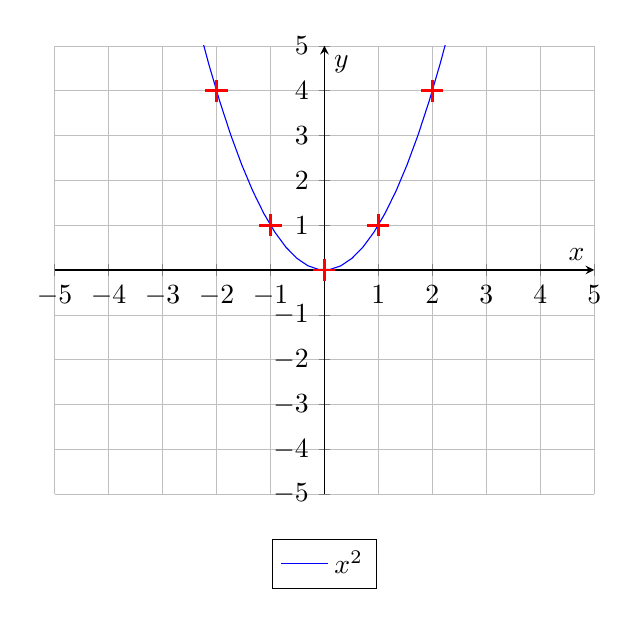
\begin{tikzpicture}%[scale=1.0]
        \begin{axis}[
                xlabel=$x$,
                ylabel=$y$,
                xmax=5,
                xmin=-5,
                ymax=5,
                ymin=-5,
                axis x line=middle,
                axis y line=middle,
                legend style={at={(0.5,-0.1)},
                        anchor=north,legend columns=-1},
                grid=major,
                grid style={line width=.1pt, draw=gray!10},
                major grid style={line width=.2pt,draw=gray!50},
                xtick={-5,-4,-3,-2,-1,0,1,2,3,4,5},
                ytick={-5,-4,-3,-2,-1,0,1,2,3,4,5},
                samples=50
            ]
            \addplot [blue] {x^2};
            \addlegendentry {$x^2$};
            \addplot+[
                mark=+,
                only marks,
                mark size=4pt,
                mark options={line width=1pt},
                mark color=red
            ]
            coordinates
                {(-2,4) (-1,1) (0,0) (1,1) (2,4)};

        \end{axis}
    \end{tikzpicture}

    \subsubsection{Normalparabel nach oben/unten verschieben}
    \vspace{-4mm}
    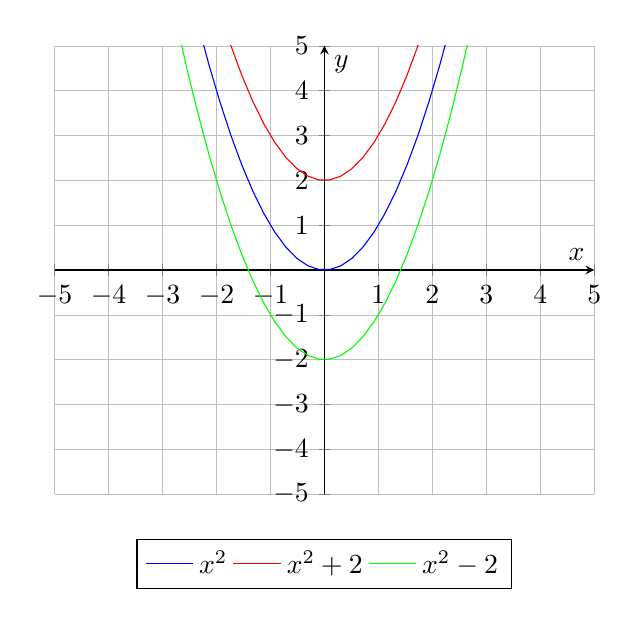
\begin{tikzpicture}%[scale=1.0]
        \begin{axis}[
                xlabel=$x$,
                ylabel=$y$,
                xmax=5,
                xmin=-5,
                ymax=5,
                ymin=-5,
                axis x line=middle,
                axis y line=middle,
                legend style={at={(0.5,-0.1)},
                        anchor=north,legend columns=-1},
                grid=major,
                grid style={line width=.1pt, draw=gray!10},
                major grid style={line width=.2pt,draw=gray!50},
                xtick={-5,-4,-3,-2,-1,0,1,2,3,4,5},
                ytick={-5,-4,-3,-2,-1,0,1,2,3,4,5},
                samples=50
            ]
            \addplot [blue] {x^2};
            \addlegendentry {$x^2$};
            \addplot [red] {x^2+2};
            \addlegendentry {$x^2+2$};
            \addplot [green] {x^2-2};
            \addlegendentry {$x^2-2$};
        \end{axis}
    \end{tikzpicture}
    \begin{equation*} {\color{red}f(x)} + c = \begin{cases} \text{ Verschiebung nach oben} &\text{für } c > 0 \\[5px] \text{ Verschiebung nach unten} &\text{für } c < 0 \end{cases} \end{equation*}


    \subsubsection{Normalparabel stauchen/strecken}
    \vspace{-4mm}
    Moechte man die Normalparabel stauchen oder strecken, muss man sich die Parabelgleichung $f(x) = ax^2$ anschauen.

    \begin{tabularx}{0.5\textwidth} {
            | >{\raggedright\arraybackslash}c
            | >{\raggedright\arraybackslash}X |}
        \hline
        $a > 1$      & Die Parabel ist nach oben geoeffnet und
        schmaler* als die Normalparabel                         \\ \hline
        $a = 1$      & Die nach oben geoeffnete Normalparabel   \\ \hline
        $0 < a < 1$  & Die Parabel ist nach oben geoeffnet und
        breiter**  als die Normalparabel                        \\ \hline
        $-1 < a < 0$ & Die Parabel ist nach unten geoeffnet und
        breiter**  als die Normalparabel                        \\ \hline
        $a = -1$     & Die nach unten geoeffnete Normalparabel  \\ \hline
        $a < -1$     & Die Parabel ist nach unten geoeffnet und
        schmaler*   als die Normalparabel                       \\ \hline
    \end{tabularx}
    \\~\\
    * gestreckt, ** gestaucht \\~\\
    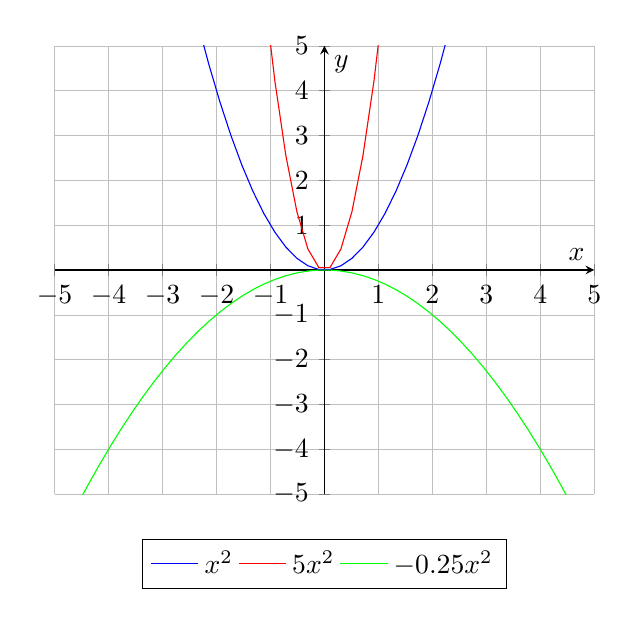
\begin{tikzpicture}%[scale=1.0]
        \begin{axis}[
                xlabel=$x$,
                ylabel=$y$,
                xmax=5,
                xmin=-5,
                ymax=5,
                ymin=-5,
                axis x line=middle,
                axis y line=middle,
                legend style={at={(0.5,-0.1)},
                        anchor=north,legend columns=-1},
                grid=major,
                grid style={line width=.1pt, draw=gray!10},
                major grid style={line width=.2pt,draw=gray!50},
                xtick={-5,-4,-3,-2,-1,0,1,2,3,4,5},
                ytick={-5,-4,-3,-2,-1,0,1,2,3,4,5},
                samples=50
            ]
            \addplot [blue] {x^2};
            \addlegendentry {$x^2$};
            \addplot [red] {5*x^2};
            \addlegendentry {$5x^2$};
            \addplot [green] {-0.25*x^2};
            \addlegendentry {$-0.25x^2$};

        \end{axis}
    \end{tikzpicture}
    \subsubsection{Parabel verschieben entlang der x-Achse}
    \vspace{-4mm}
    \begin{equation*} f({\color{red}x} + d) = \begin{cases} \text{ Verschiebung nach rechts} &\text{für } d < 0 \\[5px] \text{ Verschiebung nach links} &\text{für } d > 0 \end{cases} \end{equation*}
    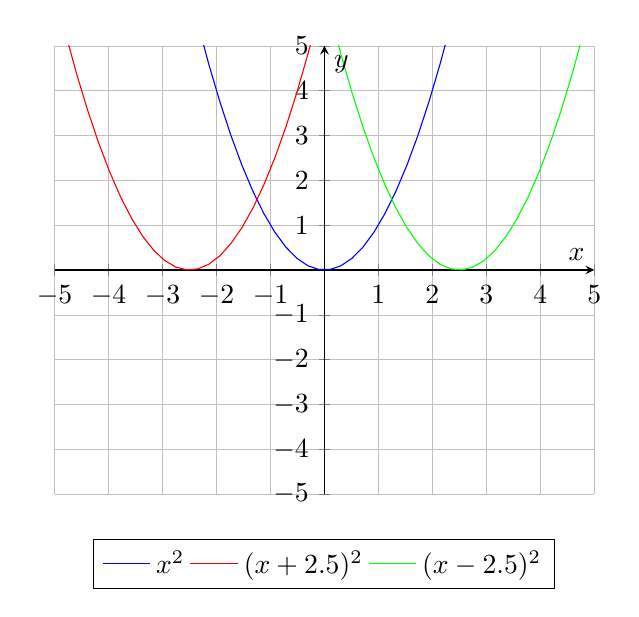
\begin{tikzpicture}%[scale=1.0]
        \begin{axis}[
                xlabel=$x$,
                ylabel=$y$,
                xmax=5,
                xmin=-5,
                ymax=5,
                ymin=-5,
                axis x line=middle,
                axis y line=middle,
                legend style={at={(0.5,-0.1)},
                        anchor=north,legend columns=-1},
                grid=major,
                grid style={line width=.1pt, draw=gray!10},
                major grid style={line width=.2pt,draw=gray!50},
                xtick={-5,-4,-3,-2,-1,0,1,2,3,4,5},
                ytick={-5,-4,-3,-2,-1,0,1,2,3,4,5},
                samples=50
            ]
            \addplot [blue] {x^2};
            \addlegendentry {$x^2$};
            \addplot [red] {(x+2.5)^2};
            \addlegendentry {$(x+2.5)^2$};
            \addplot [green] {(x-2.5)^2};
            \addlegendentry {$(x-2.5)^2$};

        \end{axis}
    \end{tikzpicture}

    \subsubsection{y-Achsenabschnitt berechnen}
    \vspace{-4mm}
    Die x-Koordinate des Schnittpunktes mit der y-Achse ist immer Null. \\
    Bei quadratischen Funktionen lässt sich der y-Achsenabschnitt aus der Funktionsgleichung ablesen: Der y-Achsenabschnitt von $y = ax^2 + bx + {\color{red}c}$ ist $y = {\color{red}c}$.
    \subsubsection{Nullstellen berechnen}
    \begin{enumerate}
        \item Funktionsgleichung gleich Null setzen
        \item Gleichung lösen
    \end{enumerate}
    Da die y-Koordinate eines Schnittpunktes mit der x-Achse immer Null ist, lautet der Ansatz zur Berechnung einer Nullstelle: $y = 0$. Wegen $y = f(x)$ kann man auch $f(x) = 0$ schreiben. \\~\\
    \textbf{Fall 1: $f(x) = ax^2$} \\~\\
    Funktionen vom Typ $f(x) = ax^2$ besitzen als einzige Nullstelle die Null. \\~\\
    \textbf{Fall 2: $f(x) = ax^2 + c$} . \\~\\
    \begin{enumerate}
        \item     Funktionsgleichung gleich Null setzen
        \item     Gleichung nach $x^2$ auflösen
        \item     Wurzel ziehen
    \end{enumerate}

    \textbf{Fall 3: $f(x) = ax^2 + bx$} . \\~\\
    \begin{enumerate}
        \item     Funktionsgleichung gleich Null setzen
        \item     Gleichung nach $x$ ausklammern
        \item     Faktoren gleich Null setzen
    \end{enumerate}

    \textbf{Fall 4: $f(x) = ax^2 + bx + c$} . \\~\\
    Quadratische Gleichungen dieses Typs lösen wir mit der Mitternachtsformel
    \subsection{Gebrochenrationale Funktionen}
    \vspace{-4mm}
    \subsubsection{Definition}
    \vspace{-4mm}
    Eine gebrochenrationale Funktion ist eine Funktion, bei der sich sowohl im Zähler als auch im Nenner eines Bruchs eine ganzrationale Funktion befindet.
    \subsubsection{Definitionsmenge}
    Die Definitionsmenge $\mathbb{D}_f$ ist die Menge aller x-Werte, die in die Funktion eingesetzt werden duerfen.

    In gebrochenrationale Funktionen duerfen wir grundsätzlich alle reellen Zahlen   ausser die, für die der Nenner gleich Null wird  einsetzen: $\mathbb{D}_f = \mathbb{R}\setminus\{\text{Nullstellen der Nennerfunktion}\}$
    \subsubsection{Senkrechte Asymptote}
    \vspace{-4mm}
    Eine senkrechte Gerade, der sich eine Kurve bei deren immer groesser werdender Entfernung vom Koordinatenursprung unbegrenzt nähert, heisst senkrechte Asymptote.\\
    \textbf{Bedingung}\\
    Bedingung für die Existenz einer senkrechten Asymptote ist, dass die Nennerfunktion (mindestens) eine Nullstelle hat:

    \textbf{Anleitung}
    Funktionsgleichung der Nennerfunktion gleich Null setzen: \\
    $f(x) = \frac{1}{x-1} \Longrightarrow x - 1 = 0$  \\
    Gleichung lösen: $x = 1$ \\
    Die senkrechte Asymptote verlauft durch x = 1.


    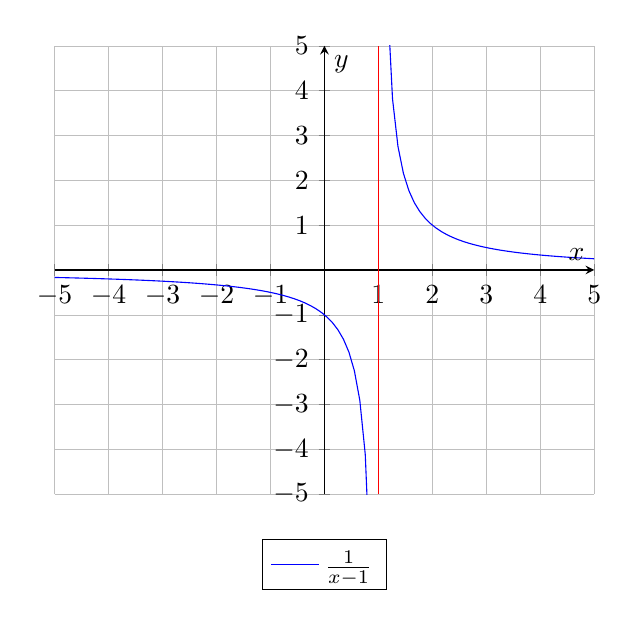
\begin{tikzpicture}%[scale=1.0]
        \begin{axis}[
                xlabel=$x$,
                ylabel=$y$,
                xmax=5,
                xmin=-5,
                ymax=5,
                ymin=-5,
                axis x line=middle,
                axis y line=middle,
                legend style={at={(0.5,-0.1)},
                        anchor=north,legend columns=-1},
                grid=major,
                grid style={line width=.1pt, draw=gray!10},
                major grid style={line width=.2pt,draw=gray!50},
                xtick={-5,-4,-3,-2,-1,0,1,2,3,4,5},
                ytick={-5,-4,-3,-2,-1,0,1,2,3,4,5},
                samples=50
            ]
            \addplot[samples=100,domain=-5:5,blue,restrict y to domain=-15:15]{1/(x-1)};
            \addlegendentry {$\frac{1}{x-1}$};
            \draw[red] ({axis cs:1,0}|-{rel axis cs:0,0}) -- ({axis cs:1,0}|-{rel axis cs:0,1});
            \addlegendentry {$x=1$};

        \end{axis}
    \end{tikzpicture}


    \subsubsection{Waagrechte Asymptote}
    \vspace{-4mm}
    Eine waagrechte Gerade, der sich eine Kurve bei deren immer groesser werdender Entfernung vom Koordinatenursprung unbegrenzt nähert, heisst waagrechte Asymptote.

    \textbf{Bedingung}\\
    Eine gebrochenrationale Funktion:
    \[y = \frac{{\color{red}a_n} x^{\fcolorbox{red}{white}{$n$}} + a_{n-1} x^{n-1} + \dots + a_1 x + a_ 0}{{\color{red}b_m} x^{\fcolorbox{red}{white}{$m$}} + b_{m-1} x^{m-1} + \dots + b_1 x + b_ 0}\]
    besitzt eine waagrechte Asymptote, wenn: \\
    Zählergrad < Nennergrad (n < m) dann: Die x-Achse ist die waagrechte Asymptote \\

    Zählergrad = Nennergrad (n = m) dann:  Die zur x-Achse parallele Gerade mit der Gleichung $y = {\color{red}\frac{a_n}{b_m}}$ ist die waagrechte Asymptote.


    \textbf{Anleitung}
    Zählergrad und Nennergrad bestimmen: \\
    Da der Zählergrad (0) kleiner ist als der Nennergrad (1), besitzt die gebrochenrationale Funktion eine waagrechte Asymptote.
    Waagrechte Asymptote berechnen: \\
    Wegen Zählergrad < Nennergrad ist die x-Achse die waagrechte Asymptote.


    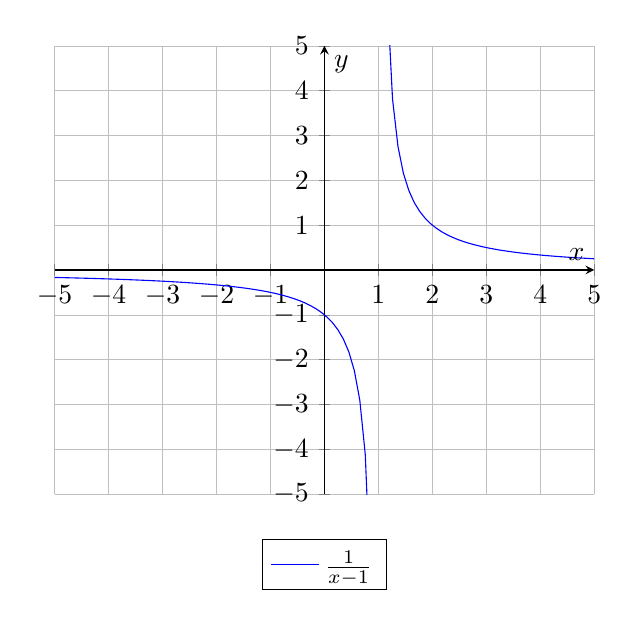
\begin{tikzpicture}%[scale=1.0]
        \begin{axis}[
                xlabel=$x$,
                ylabel=$y$,
                xmax=5,
                xmin=-5,
                ymax=5,
                ymin=-5,
                axis x line=middle,
                axis y line=middle,
                legend style={at={(0.5,-0.1)},
                        anchor=north,legend columns=-1},
                grid=major,
                grid style={line width=.1pt, draw=gray!10},
                major grid style={line width=.2pt,draw=gray!50},
                xtick={-5,-4,-3,-2,-1,0,1,2,3,4,5},
                ytick={-5,-4,-3,-2,-1,0,1,2,3,4,5},
                samples=50
            ]
            \addplot[samples=100,domain=-5:5,blue,restrict y to domain=-15:15]{1/(x-1)};
            \addlegendentry {$\frac{1}{x-1}$};
        \end{axis}
    \end{tikzpicture}

    \subsubsection{Schiefe Asymptote}
    \vspace{-4mm}
    Eine schiefe Gerade, der sich eine Kurve bei deren immer grösser werdender Entfernung vom Koordinatenursprung unbegrenzt nähert, heißt schiefe Asymptote.

    \textbf{Bedingung}\\
    Eine gebrochenrationale Funktion:
    \[y = \frac{a_n x^{\fcolorbox{red}{white}{$n$}} + a_{n-1} x^{n-1} + \dots + a_1 x + a_ 0}{b_m x^{\fcolorbox{red}{white}{$m$}} + b_{m-1} x^{m-1} + \dots + b_1 x + b_ 0}\]
    besitzt eine schiefe Asymptote, wenn: \\
    Zählergrad = Nennergrad +1 (n = m + 1)

    \textbf{Anleitung} \\
    Zählergrad und Nennergrad bestimmen: \\
    $f(x) = \frac{x^2}{x+1}$ \\
    Da der Zählergrad (2) um eine Einheit größer ist als der Nennergrad (1), besitzt die gebrochenrationale Funktion eine schiefe Asymptote. \\
    Polynomdivision: \\
    $\begin{array}{l} \quad x^2:(x+1)= {\color{red}x - 1}+ {\color{blue}\frac{1}{x+1}} \\ -(x^2 + x) \\ \qquad \quad -x \\ \qquad -(-x-1) \\ \qquad \qquad \qquad 1 \end{array}$ \\
    Grenzwertbetrachtung: \\
    Da der Nennergrad des Bruchs (ganz rechts im Ergebnis der Polynomdivison) größer ist als der Zählergrad, wird dieser Restterm für sehr grosse x-Werte immer kleiner und nähert sich Null an: \\
    $\lim_{x\to \pm\infty}\left({\color{blue}\frac{1}{x+1}}\right) = 0$ \\
    Der Graph der Funktion strebt deshalb gegen die schiefe Asymptote mit der Gleichung: $y = {\color{red}x-1}$


    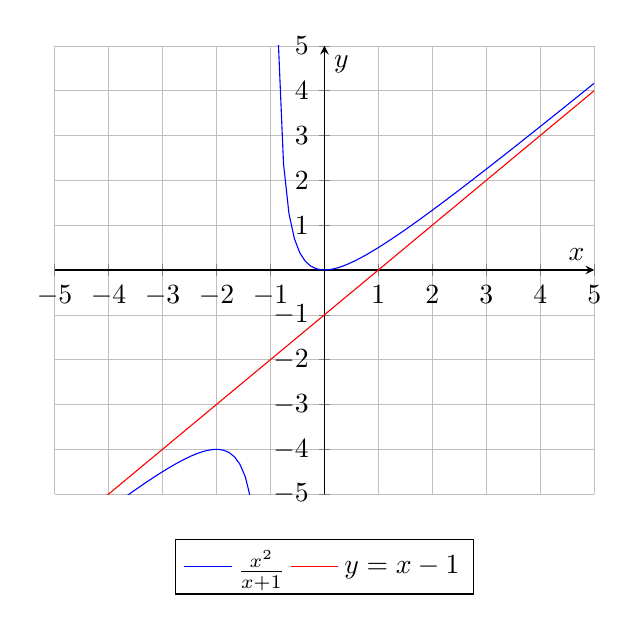
\begin{tikzpicture}%[scale=1.0]
        \begin{axis}[
                xlabel=$x$,
                ylabel=$y$,
                xmax=5,
                xmin=-5,
                ymax=5,
                ymin=-5,
                axis x line=middle,
                axis y line=middle,
                legend style={at={(0.5,-0.1)},
                        anchor=north,legend columns=-1},
                grid=major,
                grid style={line width=.1pt, draw=gray!10},
                major grid style={line width=.2pt,draw=gray!50},
                xtick={-5,-4,-3,-2,-1,0,1,2,3,4,5},
                ytick={-5,-4,-3,-2,-1,0,1,2,3,4,5},
                samples=50
            ]
            \addplot[samples=100,blue,restrict y to domain=-15:15]{x^2/(x+1)};
            \addlegendentry {$\frac{x^2}{x+1}$};
            \addplot[samples=100,domain=-5:5,red]{x-1};
            \addlegendentry {$y = x-1$};

        \end{axis}
    \end{tikzpicture}
    \subsubsection{Nullstellen}
    \vspace{-4mm}
    \begin{enumerate}
        \item Nullstellen der Zählerfunktion berechnen
              \begin{enumerate}
                  \item Funktionsgleichung gleich Null setzen
                  \item Gleichung lösen
              \end{enumerate}
        \item Nullstellen der Zählerfunktion in die Nennerfunktion einsetzen
        \item Ergebnis interpretieren
    \end{enumerate}

    \subsubsection{Polstellen}
    \vspace{-4mm}

    \begin{enumerate}
        \item Nullstellen der Nennerfunktion berechnen
              \begin{enumerate}
                  \item Funktionsgleichung gleich Null setzen
                  \item Gleichung lösen
              \end{enumerate}
        \item Nullstellen der Nennerfunktion in Zählerfunktion einsetzen
        \item Ergebnis interpretieren
    \end{enumerate}
    Wenn möglicherweise eine hebbare Definitionslücke vorliegt:
    \begin{enumerate}
        \item Zähler und Nenner faktorisieren
        \item Bruch kürzen
        \item Nullstellen der ungekürzten Nennerfunktion in gekürzte Nennerfunktion einsetzen
        \item Ergebnis interpretieren
    \end{enumerate}

    \subsection{Betragsfunktion}
    \vspace{-4mm}
    \subsubsection{Definition}
    \vspace{-4mm}
    Die Betragsfunktion ist eine abschnittsweise definierte Funktion, die sich aus zwei linearen Funktionen zusammensetzt.
    \[|x| = \begin{cases} x &\text{für } x \geq 0 \\[5px] -x &\text{für } x < 0 \end{cases}\]

    Definitionsmenge: $\mathbb{D}_f = \mathbb{R}$ \\
    Wertemenge: $\mathbb{W}_f = \mathbb{R}^{+}$

    \subsubsection{Verschiebung}
    \vspace{-4mm}
    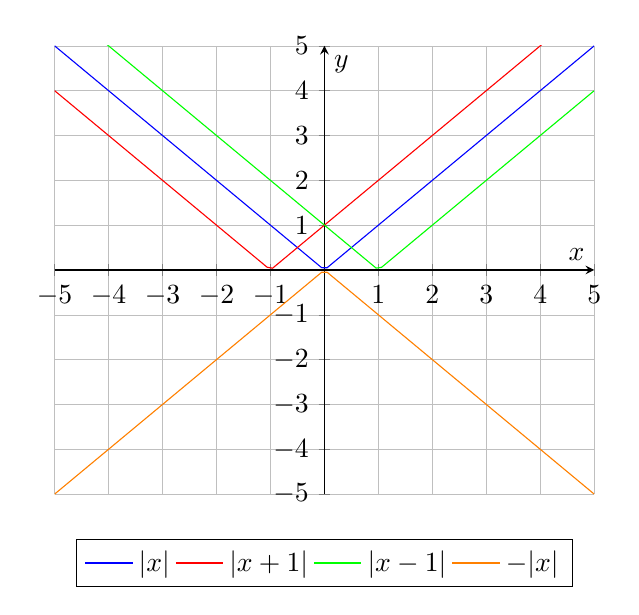
\begin{tikzpicture}%[scale=1.0]
        \begin{axis}[
                xlabel=$x$,
                ylabel=$y$,
                xmax=5,
                xmin=-5,
                ymax=5,
                ymin=-5,
                axis x line=middle,
                axis y line=middle,
                legend style={at={(0.5,-0.1)},
                        anchor=north,legend columns=-1},
                grid=major,
                grid style={line width=.1pt, draw=gray!10},
                major grid style={line width=.2pt,draw=gray!50},
                xtick={-5,-4,-3,-2,-1,0,1,2,3,4,5},
                ytick={-5,-4,-3,-2,-1,0,1,2,3,4,5},
                samples=50
            ]
            \addplot[samples=100,blue]{abs(x)};
            \addlegendentry {$|x|$};
            \addplot[samples=100,red]{abs(x+1)};
            \addlegendentry {$|x+1|$};
            \addplot[samples=100,green]{abs(x-1)};
            \addlegendentry {$|x-1|$};
            \addplot[samples=100,orange]{-abs(x)};
            \addlegendentry {$-|x|$};

        \end{axis}
    \end{tikzpicture}


    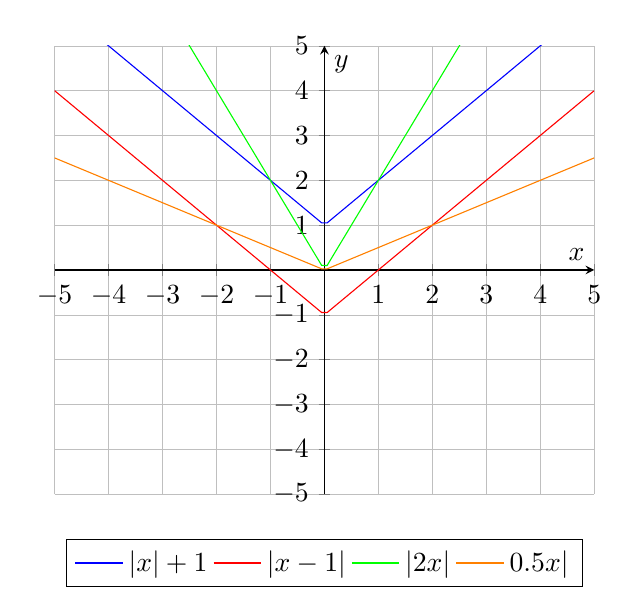
\begin{tikzpicture}%[scale=1.0]
        \begin{axis}[
                xlabel=$x$,
                ylabel=$y$,
                xmax=5,
                xmin=-5,
                ymax=5,
                ymin=-5,
                axis x line=middle,
                axis y line=middle,
                legend style={at={(0.5,-0.1)},
                        anchor=north,legend columns=-1},
                grid=major,
                grid style={line width=.1pt, draw=gray!10},
                major grid style={line width=.2pt,draw=gray!50},
                xtick={-5,-4,-3,-2,-1,0,1,2,3,4,5},
                ytick={-5,-4,-3,-2,-1,0,1,2,3,4,5},
                samples=50
            ]
            \addplot[samples=100,blue]{abs(x)+1};
            \addlegendentry {$|x|+1$};
            \addplot[samples=100,red]{abs(x)-1};
            \addlegendentry {$|x-1|$};
            \addplot[samples=100,green]{abs(2*x)};
            \addlegendentry {$|2x|$};
            \addplot[samples=100,orange]{abs(0.5*x)};
            \addlegendentry {$0.5x|$};

        \end{axis}
    \end{tikzpicture}

    \subsection{Potenzfunktionen mit Positiven Exponenten}
    \vspace{-4mm}
    \subsubsection{Definition}
    \vspace{-4mm}
    Eine Funktion $f$ mit der Funktionsgleichung $f(x) = x^n \quad \text{ mit } n \in \mathbb{Z}\setminus\{0\}$ heisst Potenzfunktion. \\~\\
    \subsubsection{Gerade Exponenten}
    \vspace{-4mm}
    Als Beispiele dienen die Funktionen $f(x) = x^2$ und $f(x) = x^4$. \\
    Um die Graphen besser zu zeichnen, berechnen wir zunächst einige Funktionswerte:
    \[\begin{array}{r|c|c|c|c|c|c|c} x & -1{,}5 & {\color{blue}-1} & -0{,}5 & {\color{blue}0} & 0{,}5 & {\color{blue}1} & 1{,}5 \\ \hline x^2 & 2{,}25 & {\color{blue}1} & 0{,}25 & {\color{blue}0} & 0{,}25 & {\color{blue}1} & 2{,}25 \\ \hline x^4 & 5{,}0625 & {\color{blue}1} & 0{,}0625 & {\color{blue}0} & 0{,}0625 & {\color{blue}1} & 5{,}0625 \end{array}\]
    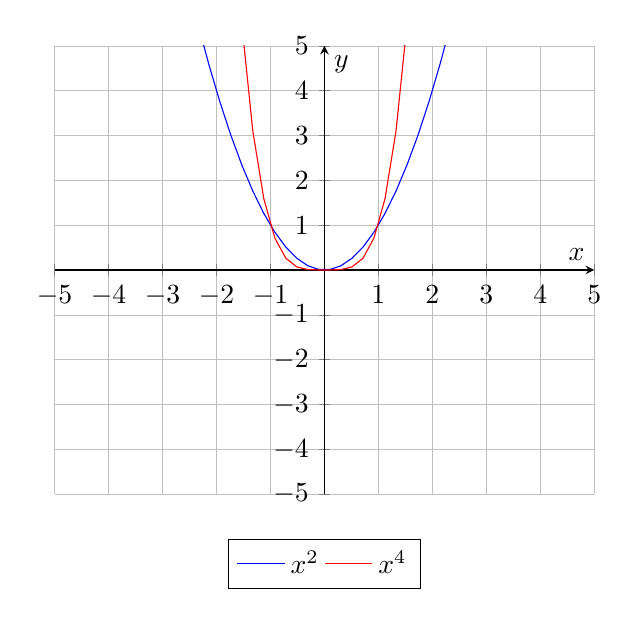
\begin{tikzpicture}%[scale=1.0]
        \begin{axis}[
                xlabel=$x$,
                ylabel=$y$,
                xmax=5,
                xmin=-5,
                ymax=5,
                ymin=-5,
                axis x line=middle,
                axis y line=middle,
                legend style={at={(0.5,-0.1)},
                        anchor=north,legend columns=-1},
                grid=major,
                grid style={line width=.1pt, draw=gray!10},
                major grid style={line width=.2pt,draw=gray!50},
                xtick={-5,-4,-3,-2,-1,0,1,2,3,4,5},
                ytick={-5,-4,-3,-2,-1,0,1,2,3,4,5},
                samples=50
            ]
            \addplot [blue] {x^2};
            \addlegendentry {$x^2$};
            \addplot [red] {x^4};
            \addlegendentry {$x^4$};


        \end{axis}
    \end{tikzpicture}
    \subsubsection{Ungerade Exponenten}
    \vspace{-4mm}
    Als Beispiele dienen die Funktionen $f(x) = x^3$ und $f(x) = x^5$. \\
    Um die Graphen besser zu zeichnen, berechnen wir zunächst einige Funktionswerte:  \

    \[\begin{array}{r|c|c|c|c|c|c|c} x & -1{,}5 & {\color{blue}-1} & -0{,}5 & {\color{blue}0} & 0{,}5 & {\color{blue}1} & 1{,}5 \\ \hline x^3 & -3{,}375 & {\color{blue}-1} & -0{,}125 & {\color{blue}0} & 0{,}125 & {\color{blue}1} & 3{,}375 \\ \hline x^5 & -7{,}59375 & {\color{blue}-1} & 0{,}03125 & {\color{blue}0} & 0{,}03125 & {\color{blue}1} & 7{,}59375 \end{array}\]
    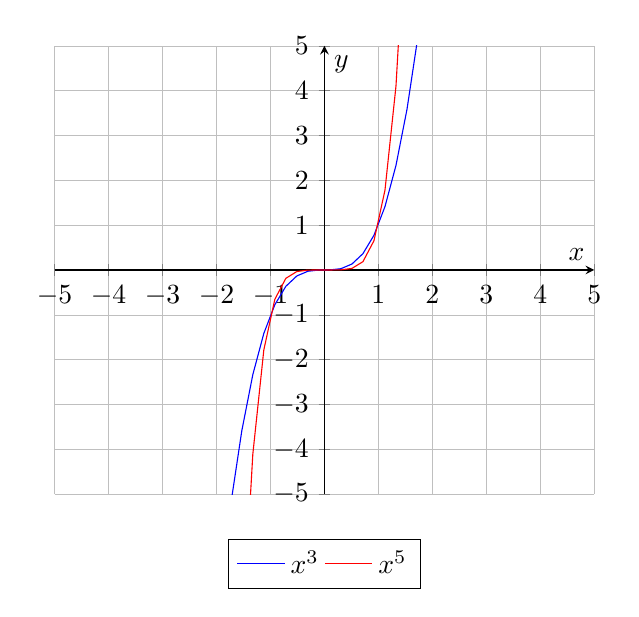
\begin{tikzpicture}%[scale=1.0]
        \begin{axis}[
                xlabel=$x$,
                ylabel=$y$,
                xmax=5,
                xmin=-5,
                ymax=5,
                ymin=-5,
                restrict y to domain=-10:10,
                axis x line=middle,
                axis y line=middle,
                legend style={at={(0.5,-0.1)},
                        anchor=north,legend columns=-1},
                grid=major,
                grid style={line width=.1pt, draw=gray!10},
                major grid style={line width=.2pt,draw=gray!50},
                xtick={-5,-4,-3,-2,-1,0,1,2,3,4,5},
                ytick={-5,-4,-3,-2,-1,0,1,2,3,4,5},
                samples=50
            ]
            \addplot [blue] {x^3};
            \addlegendentry {$x^3$};
            \addplot [red] {x^5};
            \addlegendentry {$x^5$};
        \end{axis}
    \end{tikzpicture}

    \subsubsection{Zusammenfassung der wichtigsten Eigenschaften}
    \vspace{-4mm}
    Potenzfunktionen mit positiven ganzzahligen Exponenten $\boldsymbol{f(x) = x^n}$ haben folgende Eigenschaften:
    \begin{tabularx}{0.5\textwidth} {
            | >{\raggedright\arraybackslash}X
            | >{\raggedright\arraybackslash}X
            | >{\raggedright\arraybackslash}X |}
        \hline
                          & \textbf{n gerade}                 & \textbf{n ungerade}       \\ \hline
        Definitionsmenge  & $\mathbb{D} = \mathbb{R}$         & $\mathbb{D} = \mathbb{R}$ \\ \hline
        Wertemenge        & $\mathbb{W} = \mathbb{R}^{+}_{0}$ & $\mathbb{W} = \mathbb{R}$ \\ \hline
        Symmetrie         & achsensymmetrisch                 & punktsymetrisch           \\
                          & zur y-ache                        & zum K-Ursprung            \\ \hline
        Gemeinsame Punkte & $(-1,1)$,$(0|0)$,$(1|1)$          & $(-1,-1)$,$(0|0)$,$(1|1)$ \\ \hline
    \end{tabularx}
    \subsection{Potenzfunktionen mit negativen Exponenten}
    \vspace{-4mm}
    Die Graphen von Potenzfunktionen heissen Hyperbeln n-ter Ordnung, wenn der Exponent negativ ist.
    \subsubsection{Gerade Exponenten}
    \vspace{-4mm}
    Als Beispiele dienen die Funktionen $f(x) = x^{-2}$ und $f(x) = x^{-4}$. \\
    Um die Graphen besser zu zeichnen, berechnen wir zunächst einige Funktionswerte: \\~\\
    $\begin{array}{r|c|c|c|c|c|c} x & -1{,}5 & {\color{blue}-1} & -0{,}5 & 0{,}5 & {\color{blue}1} & 1{,}5 \\ \hline x^{-2} & 0{,}\bar{4} & {\color{blue}1} & 4 & 4 & {\color{blue}1} & 0{,}\bar{4} \\ \hline x^{-4} & \approx 0{,}1975 & {\color{blue}1} & 16 & 16 & {\color{blue}1} & \approx 0{,}1975 \end{array}$ \\~\\
    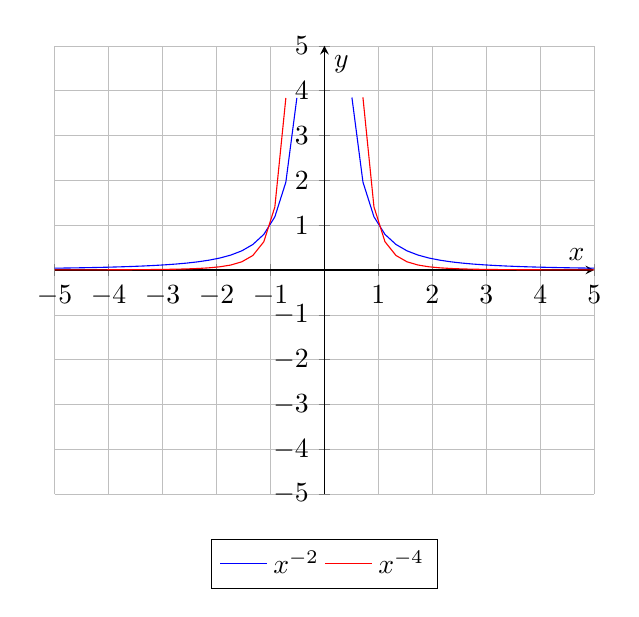
\begin{tikzpicture}%[scale=1.0]
        \begin{axis}[
                xlabel=$x$,
                ylabel=$y$,
                xmax=5,
                xmin=-5,
                ymax=5,
                ymin=-5,
                restrict y to domain=-10:10,
                axis x line=middle,
                axis y line=middle,
                legend style={at={(0.5,-0.1)},
                        anchor=north,legend columns=-1},
                grid=major,
                grid style={line width=.1pt, draw=gray!10},
                major grid style={line width=.2pt,draw=gray!50},
                xtick={-5,-4,-3,-2,-1,0,1,2,3,4,5},
                ytick={-5,-4,-3,-2,-1,0,1,2,3,4,5},
                samples=50
            ]
            \addplot [blue] {x^-2};
            \addlegendentry {$x^{-2}$};
            \addplot [red] {x^-4};
            \addlegendentry {$x^{-4}$};
        \end{axis}
    \end{tikzpicture}
    \subsubsection{Gerade Exponenten}
    \vspace{-4mm}
    Als Beispiele dienen die Funktionen $f(x) = x^{-3}$ und $f(x) = x^{-5}$. \\
    Um die Graphen besser zu zeichnen, berechnen wir zunächst einige Funktionswerte: \\~\\
    $\begin{array}{r|c|c|c|c|c|c} x & -1{,}5 & {\color{blue}-1} & -0{,}5 & 0{,}5 & {\color{blue}1} & 1{,}5 \\ \hline x^{-3} & \approx -0{,}2963 & {\color{blue}-1} & -8 & 8 & {\color{blue}1} & \approx 0{,}2963 \\ \hline x^{-5} & \approx -0{,}1317 & {\color{blue}-1} & -32 & 32 & {\color{blue}1} & \approx 0{,}1317 \end{array}$ \\~\\
    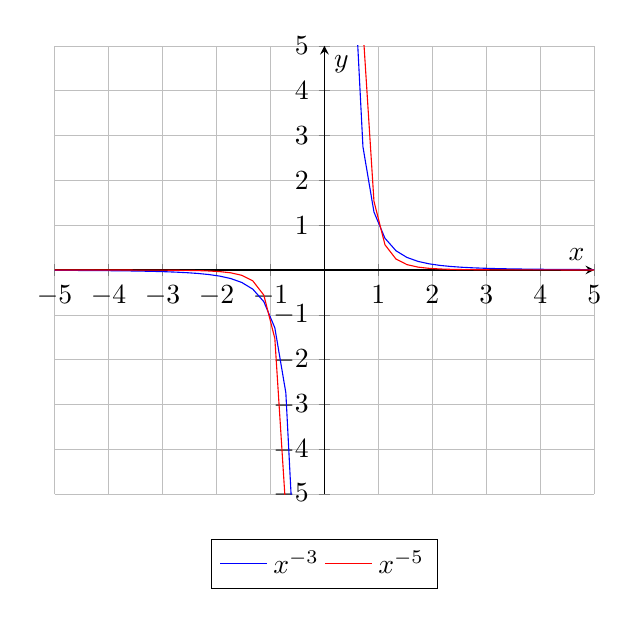
\begin{tikzpicture}%[scale=1.0]
        \begin{axis}[
                xlabel=$x$,
                ylabel=$y$,
                xmax=5,
                xmin=-5,
                ymax=5,
                ymin=-5,
                restrict y to domain=-10:10,
                axis x line=middle,
                axis y line=middle,
                legend style={at={(0.5,-0.1)},
                        anchor=north,legend columns=-1},
                grid=major,
                grid style={line width=.1pt, draw=gray!10},
                major grid style={line width=.2pt,draw=gray!50},
                xtick={-5,-4,-3,-2,-1,0,1,2,3,4,5},
                ytick={-5,-4,-3,-2,-1,0,1,2,3,4,5},
                samples=50
            ]
            \addplot [blue] {x^-3};
            \addlegendentry {$x^{-3}$};
            \addplot [red] {x^-5};
            \addlegendentry {$x^{-5}$};
        \end{axis}
    \end{tikzpicture}

    \subsubsection{Zusammenfassung der wichtigsten Eigenschaften}
    \vspace{-4mm}
    Potenzfunktionen mit negativen ganzzahligen Exponenten $\boldsymbol{f(x) = x^{-n}}$ haben folgende Eigenschaften:
    \begin{tabularx}{0.5\textwidth} {
            | >{\raggedright\arraybackslash}X
            | >{\raggedright\arraybackslash}X
            | >{\raggedright\arraybackslash}X |}
        \hline
                          & \textbf{n gerade}                       & \textbf{n ungerade}                     \\ \hline
        Definitionsmenge  & $\mathbb{D} = \mathbb{R}\setminus\{0\}$ & $\mathbb{D} = \mathbb{R}\setminus\{0\}$ \\ \hline
        Wertemenge        & $\mathbb{W} = \mathbb{R}^{+}$           & $\mathbb{W} = \mathbb{R}\setminus\{0\}$ \\ \hline
        Symmetrie         & achsensymmetrisch                       & punktsymetrisch                         \\
                          & zur y-ache                              & zum K-Ursprung                          \\ \hline
        Gemeinsame Punkte & $(-1,1)$,$(1|1)$                        & $(-1,-1)$,$(1|1)$                       \\ \hline
        Asymptoten        & x-Achse, y-Achse                        & x-Achse, y-Achse                        \\ \hline
    \end{tabularx}


    \subsection{Wurzelfunktion}
    \vspace{-4mm}
    \subsubsection{Definition}
    \vspace{-4mm}
    Wurzelfunktionen sind die Umkehrfunktionen von Potenzfunktionen.
    Die Eigenschaften der Funktionen unterscheiden sich danach, ob die (Wurzel-)Exponenten gerade oder ungerade sind.

    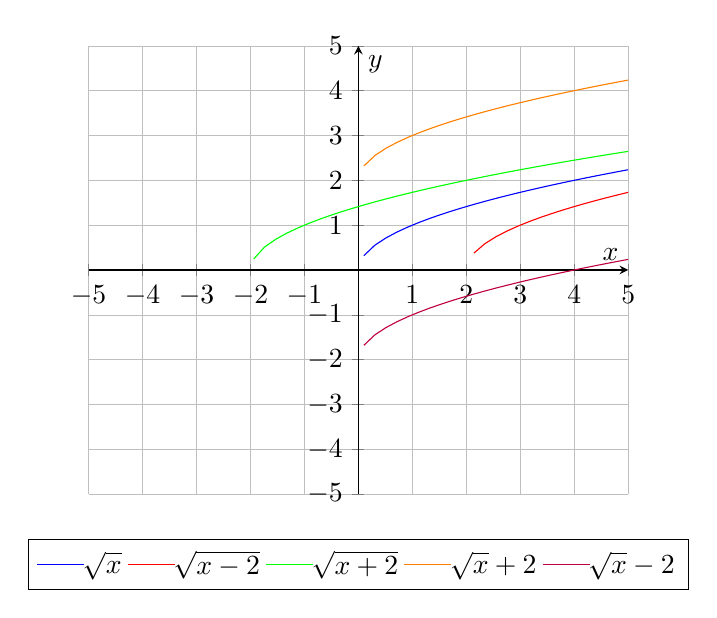
\begin{tikzpicture}%[scale=1.0]
        \begin{axis}[
                xlabel=$x$,
                ylabel=$y$,
                xmax=5,
                xmin=-5,
                ymax=5,
                ymin=-5,
                restrict y to domain=-10:10,
                axis x line=middle,
                axis y line=middle,
                legend style={at={(0.5,-0.1)},
                        anchor=north,legend columns=-1},
                grid=major,
                grid style={line width=.1pt, draw=gray!10},
                major grid style={line width=.2pt,draw=gray!50},
                xtick={-5,-4,-3,-2,-1,0,1,2,3,4,5},
                ytick={-5,-4,-3,-2,-1,0,1,2,3,4,5},
                samples=50
            ]
            \addplot [blue] {sqrt(x)};
            \addlegendentry {$\sqrt[]{x}$};
            \addplot [red] {sqrt(x-2)};
            \addlegendentry {$\sqrt[]{x-2}$};
            \addplot [green] {sqrt(x+2)};
            \addlegendentry {$\sqrt[]{x+2}$};
            \addplot [orange] {sqrt(x)+2};
            \addlegendentry {$\sqrt[]{x}+2$};
            \addplot [purple] {sqrt(x)-2};
            \addlegendentry {$\sqrt[]{x}-2$};

        \end{axis}
    \end{tikzpicture}


    \subsection{Exponentialfunktion}
    \vspace{-4mm}
    \subsubsection{Definition}
    \vspace{-4mm}
    Eine Funktion mit der Funktionsgleichung $y = a^x \quad \text{ mit } a \in \mathbb{R}^{+}\setminus\{1\}$ heisst Exponentialfunktion.

    \begin{tabularx}{0.5\textwidth} {
            | >{\raggedright\arraybackslash}X
            | >{\raggedright\arraybackslash}X |}
        \hline
        Funktionsgleichung        & $f(x) = a^x \quad \text{mit } a \in \mathbb{R}^{+}\setminus\{1\}$ \\ \hline
        Definitionsmenge          & $\mathbb{D} = \mathbb{R}$                                         \\ \hline
        Wertemenge                & $\mathbb{W} = \mathbb{R}^{+}$                                     \\ \hline
        Asymptote                 & $y = 0$ (x-Achse)                                                 \\ \hline
        Schnittpunkt mit y-Achse  & $P(0|1)$ wegen $f(0) = a^0 = 1$                                   \\ \hline
        Schnittpunkte mit x-Achse & Es gibt keine                                                     \\ \hline
        Monotonie                 & streng monoton $0 < a < 1$  = fallend $a > 1$ = steigend          \\ \hline
        Umkehrfunktion            & $f(x) = \log_{a}x$ Logarithmusfunktion                            \\ \hline
    \end{tabularx}

    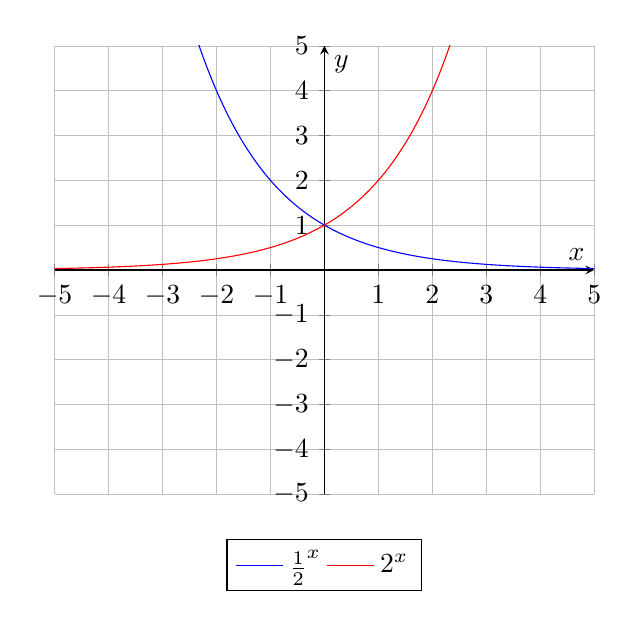
\begin{tikzpicture}%[scale=1.0]
        \begin{axis}[
                xlabel=$x$,
                ylabel=$y$,
                xmax=5,
                xmin=-5,
                ymax=5,
                ymin=-5,
                restrict y to domain=-10:10,
                axis x line=middle,
                axis y line=middle,
                legend style={at={(0.5,-0.1)},
                        anchor=north,legend columns=-1},
                grid=major,
                grid style={line width=.1pt, draw=gray!10},
                major grid style={line width=.2pt,draw=gray!50},
                xtick={-5,-4,-3,-2,-1,0,1,2,3,4,5},
                ytick={-5,-4,-3,-2,-1,0,1,2,3,4,5},
                samples=200
            ]
            \addplot [blue] {(1/2)^x};
            \addlegendentry {$\frac{1}{2}^x$};
            \addplot [red] {2^x};
            \addlegendentry {$2^x$};
        \end{axis}
    \end{tikzpicture}

    Alle Exponentialkurven verlaufen oberhalb der x-Achse. \\
    Alle Exponentialkurven schneiden die y-Achse im Punkt $(0|1)$ . $\Longrightarrow$ Laut einem Potenzgesetz gilt nämlich: $a^0 = 1$ \\
    Exponentialkurven haben keinen Schnittpunkt mit der x-Achse.
    \subsection{Logarithmusfunktion}
    \vspace{-4mm}
    \subsubsection{Definition}
    \vspace{-4mm}
    Eine Funktion mit der Funktionsgleichung $y = \log_{a}x \quad \text{ mit } a \in \mathbb{R}^{+}\setminus\{1\}$ heisst Logarithmusfunktion.
    \begin{tabularx}{0.5\textwidth} {
            | >{\raggedright\arraybackslash}X
            | >{\raggedright\arraybackslash}X |}
        \hline
        Funktionsgleichung        & $f(x) = \log_{a}x$                                       \\ \hline
        Definitionsmenge          & $\mathbb{D} = \mathbb{R}^{+}$                            \\ \hline
        Wertemenge                & $\mathbb{W} = \mathbb{R}$                                \\ \hline
        Asymptote                 & $x = 0$ (y-Achse)                                        \\ \hline
        Schnittpunkt mit x-Achse  & $P(1|0)$                                                 \\ \hline
        Schnittpunkte mit y-Achse & Es gibt keine                                            \\ \hline
        Monotonie                 & streng monoton $0 < a < 1$  = fallend $a > 1$ = steigend \\ \hline
    \end{tabularx}

    Alle Logarithmuskurven verlaufen rechts von der y-Achse \\
    Alle Logarithmuskurven kommen der y-Achse beliebig nahe. $\Rightarrow$ Die y-Achse ist die senkrechte asymptote der Logarithmuskurve. \\
    Die Logarithmusfunktionen $f(x) = \log_{\frac{1}{a}}$ und $g(x) = \log_{a}x$ sind achsensymmetrisch zur x-Achse.

    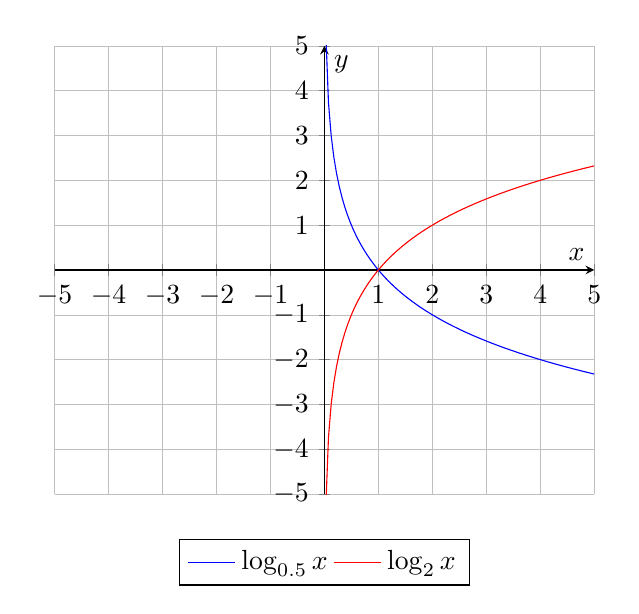
\begin{tikzpicture}%[scale=1.0]
        \begin{axis}[
                xlabel=$x$,
                ylabel=$y$,
                xmax=5,
                xmin=-5,
                ymax=5,
                ymin=-5,
                restrict y to domain=-10:10,
                axis x line=middle,
                axis y line=middle,
                legend style={at={(0.5,-0.1)},
                        anchor=north,legend columns=-1},
                grid=major,
                grid style={line width=.1pt, draw=gray!10},
                major grid style={line width=.2pt,draw=gray!50},
                xtick={-5,-4,-3,-2,-1,0,1,2,3,4,5},
                ytick={-5,-4,-3,-2,-1,0,1,2,3,4,5},
                samples=200
            ]
            \addplot [blue] {ln(x)/ln(0.5)};
            \addlegendentry {$\log_{0.5}x$};
            \addplot [red] {log2(x)};
            \addlegendentry {$\log_{2}x$};
        \end{axis}
    \end{tikzpicture}
    \newpage

\end{multicols}


\newpage{}

\section{Trigonometrie}
\subsection{Gradmass, Bogenmass}
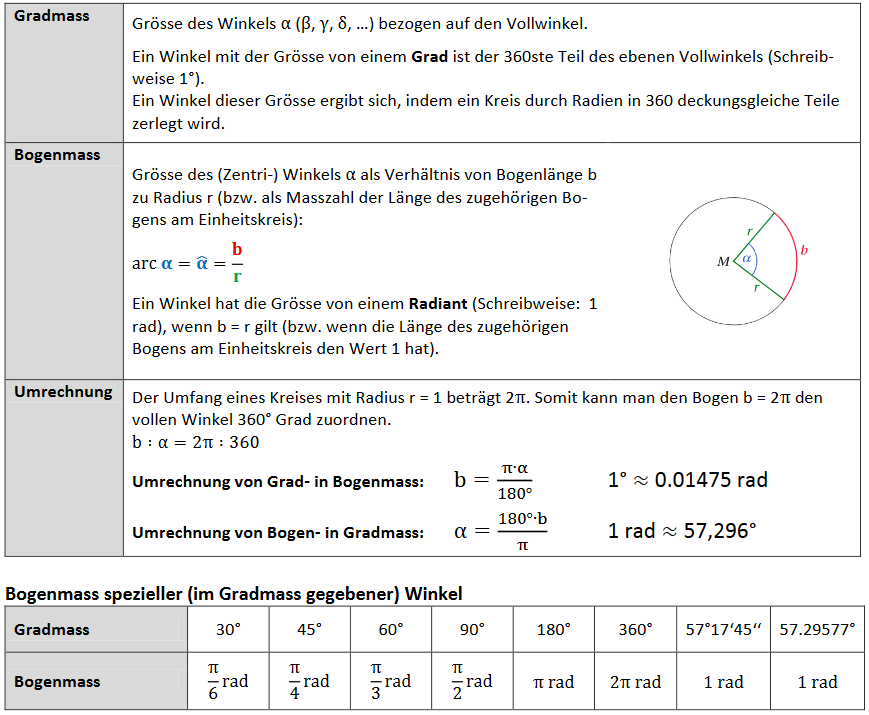
\includegraphics[scale=0.7]{gradmass.PNG}
\subsection{Trigonometrische Funktionen am rechtwinkligen Dreieck}
\subsubsection{Sinus, Kosekans}
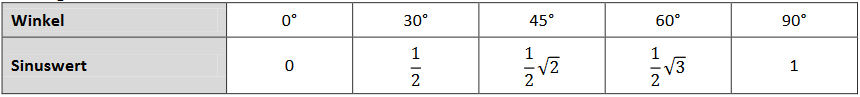
\includegraphics[scale=0.7]{sinkan1.PNG}

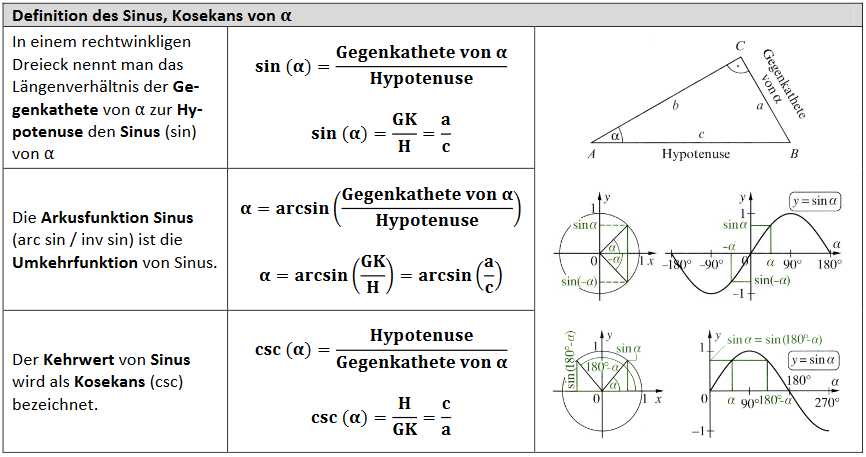
\includegraphics[scale=0.7]{sinkan2.PNG}
\subsubsection{Kosinus, Sekans}
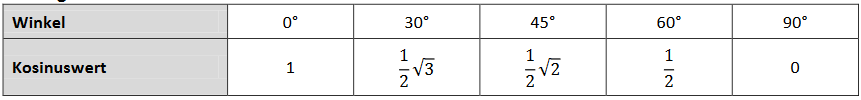
\includegraphics[scale=0.7]{kossek1.PNG}

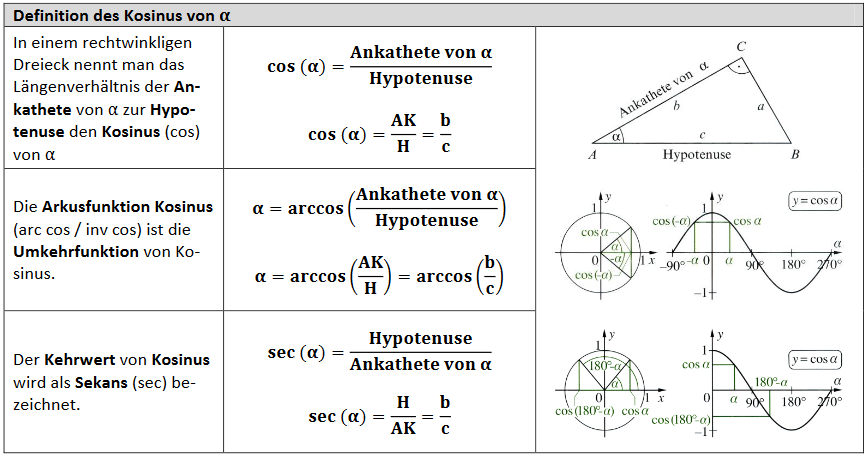
\includegraphics[scale=0.7]{kossek2.PNG}
\subsubsection{Tangens, Kotangens}
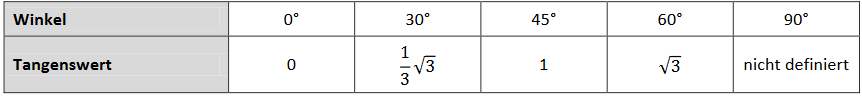
\includegraphics[scale=0.7]{tanko1.PNG}

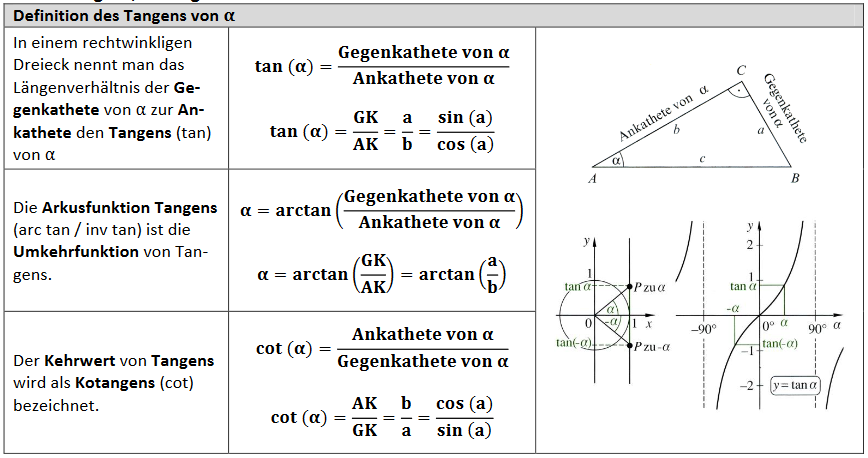
\includegraphics[scale=0.7]{tanko2.PNG}

\subsubsection{Sinus- Kosinus- und Tangensfunktion am rechtwinkligen Dreieck}
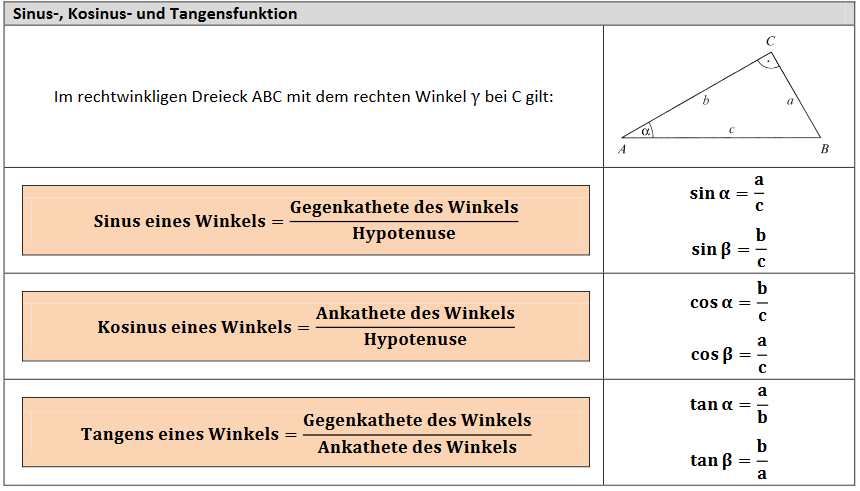
\includegraphics[scale=0.7]{sinkota.PNG}

\newpage{}


\subsection{Trigonometrische Funktionen am schiefwinkligen Dreieck}
\subsubsection{Kosinussatz}
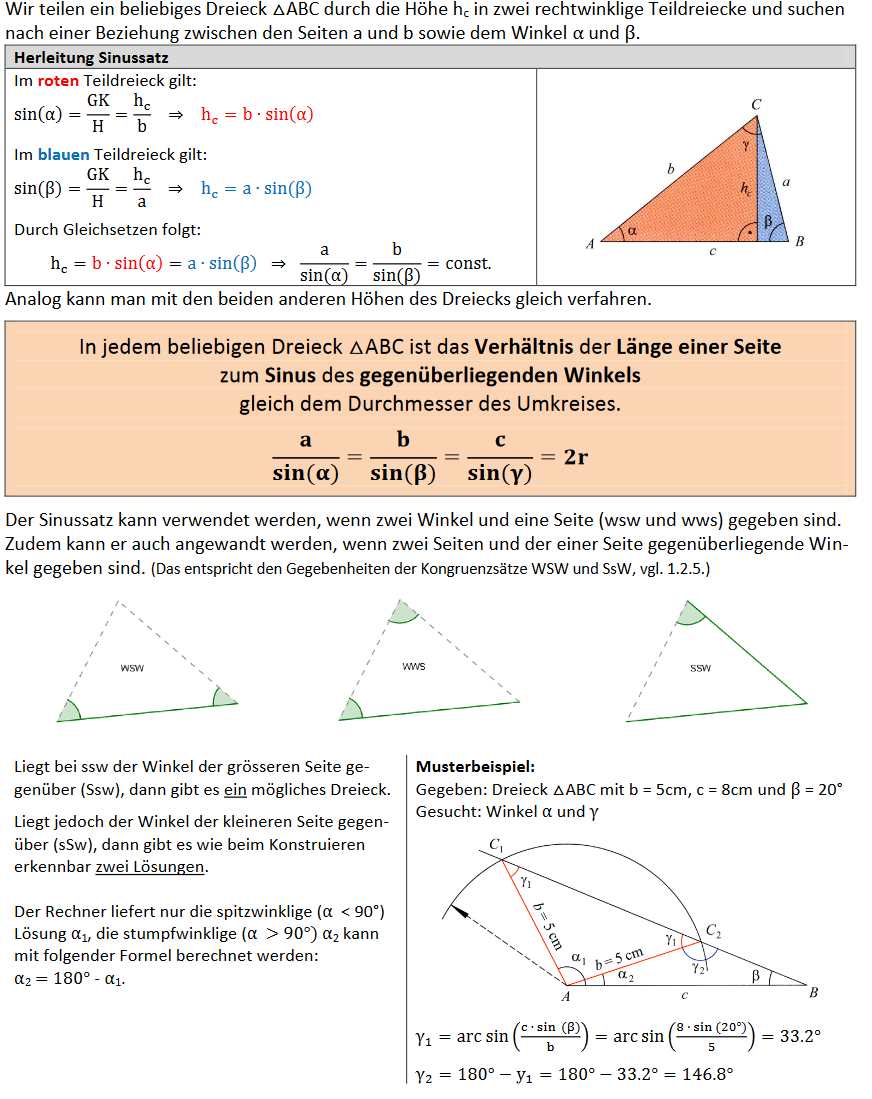
\includegraphics[scale=0.7]{sinussatz.PNG}
\subsubsection{Sinussatz}
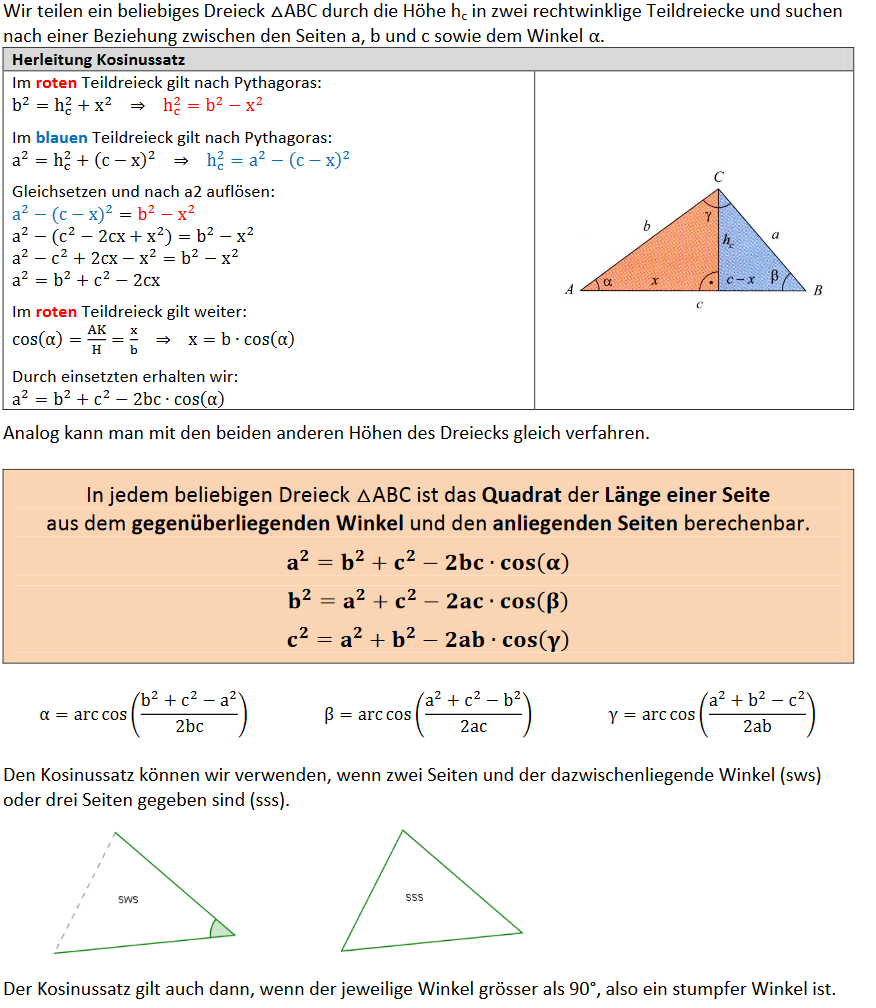
\includegraphics[scale=0.7]{kosinussatz.PNG}

\subsubsection{Flaechensatz}
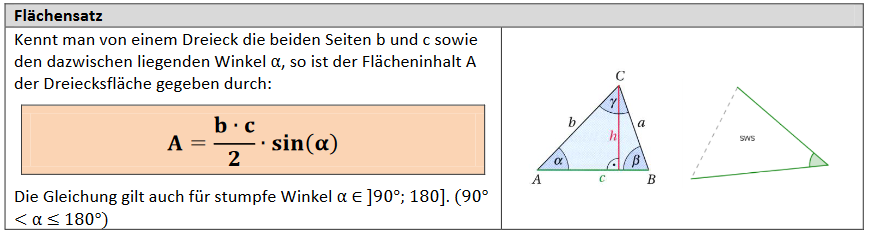
\includegraphics[scale=0.7]{flaechensatz.PNG}
\subsubsection{Berechnung am Kreissektor (auch Kreisausschnitt)}
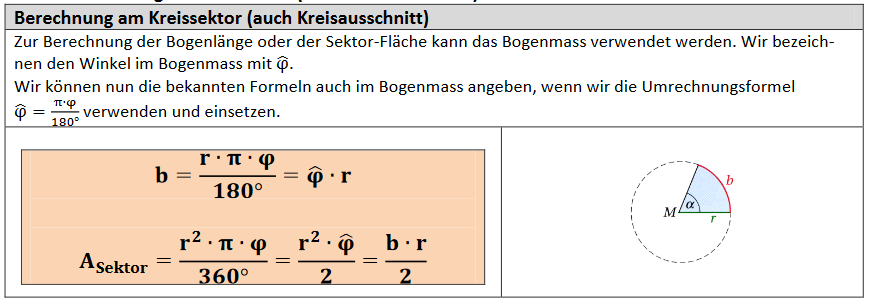
\includegraphics[scale=0.7]{kreissektor.PNG}
\subsubsection{Kreissegment (auch Kreisabschnitt)}
\includegraphics[scale=0.7]{kreissegment.PNG}



\subsection{Einheitskreis}
\subsubsection{Definition}
Der Einheitskreis ist ein Kreis um den Koordinatenursprung mit dem Radius r = 1 Längeneinheit.
\subsubsection{Beziehungen zwischen den Winkelfunktionen (Phytagoras am Einheitskreis)}
\begin{multicols}{2}
  Pythagoras am Einheitskreis:
  \[\sin^2(a)+\cos^2(a)=1\]
  Ähnlichkeiten am Einheitskreis:
  \[\tan(a)=\frac{\sin(a)}{\cos(a)}\]
  \[\cot(a)=\frac{\cos(a)}{\sin(a)}\]
  \[\tan(a)+\cot(a)=1\]


  \begin{tikzpicture}[scale=1.9]
    \draw[step=.5cm,gray,very thin] (-1.4,-1.4) grid (1.4,1.4);
    \filldraw[fill=blue!20,draw=red] (0,0) -- (3mm,0mm)
    arc [start angle=0, end angle=30, radius=3mm] -- cycle;
    \node[red] at (15:2mm) {$\alpha$};
    \draw[->] (-1.5,0) -- (1.5,0) coordinate (x axis)node[right]{$0^\circ $};
    \draw[->] (0,-1.5) -- (0,1.5) coordinate (y axis)node[above]{$90^\circ$};
    \draw[->] (1.5,0) -- (-1.5,0) coordinate (x axis)node[left]{$180^\circ$};
    \draw[->] (0,1.5) -- (0,-1.5) coordinate (y axis)node[below]{$270^\circ$};
    \draw (0,0) circle [radius=1cm];
    \draw[very thick,orange]
    (30:1cm) -- node[left=1pt,fill=white] {$\sin \alpha$} (30:1cm |- x axis);
    \draw[very thick,blue]
    (30:1cm |- x axis) -- node[below=2pt,fill=white] {$\cos \alpha$} (0,0);
    \path [name path=upward line] (1,0) -- (1,1);
    \path [name path=sloped line] (0,0) -- (30:1.5cm);
    \draw [name intersections={of=upward line and sloped line, by=t}]
    [very thick,red] (1,0) -- node [right=1pt,fill=white]
    {$\displaystyle \tan \alpha$} (t);
    \draw (0,0) -- (t);

  \end{tikzpicture}
\end{multicols}
\begin{tabularx}{1\textwidth} {
    | >{\raggedright\arraybackslash}c
    | >{\raggedright\arraybackslash}X
    | >{\raggedright\arraybackslash}X
    | >{\raggedright\arraybackslash}X
    | >{\raggedright\arraybackslash}X |}
  \hline
                      & \boldmath $\sin(a)$                    & \boldmath $\cos(a)$                    & \boldmath $\tan(a)$                    & \boldmath $\cot(a)$                    \\\hline
  \boldmath $\sin(a)$ &                                        & $\sqrt[]{1-\cos^2(a)}$                 & $\frac{\tan(a)}{\sqrt[]{1+\tan^2(a)}}$ & $\frac{1}{\sqrt[]{1+\cot^2(a)}}$       \\ \hline
  \boldmath $\cos(a)$ & $\sqrt[]{1-\sin^2(a)}$                 &                                        & $\frac{1}{\sqrt[]{1+\tan^2(a)}}$       & $\frac{\cot(a)}{\sqrt[]{1+\cot^2(a)}}$ \\ \hline
  \boldmath $\tan(a)$ & $\frac{\sin(a)}{\sqrt[]{1-\sin^2(a)}}$ & $\frac{\sqrt[]{1-\cos^2(a)}}{\cos(a)}$ &                                        & $\frac{1}{\cot(a)}$                    \\ \hline
  \boldmath $\cot(a)$ & $\frac{\sqrt[]{1-\sin^2(a)}}{\sin(a)}$ & $\frac{\cos(a)}{\sqrt[]{1-\cos^2(a)}}$ & $\frac{1}{\tan(a)}$                    &                                        \\ \hline
\end{tabularx}
\subsubsection{Vorzeichen der Trigonometrischen Funktionen}
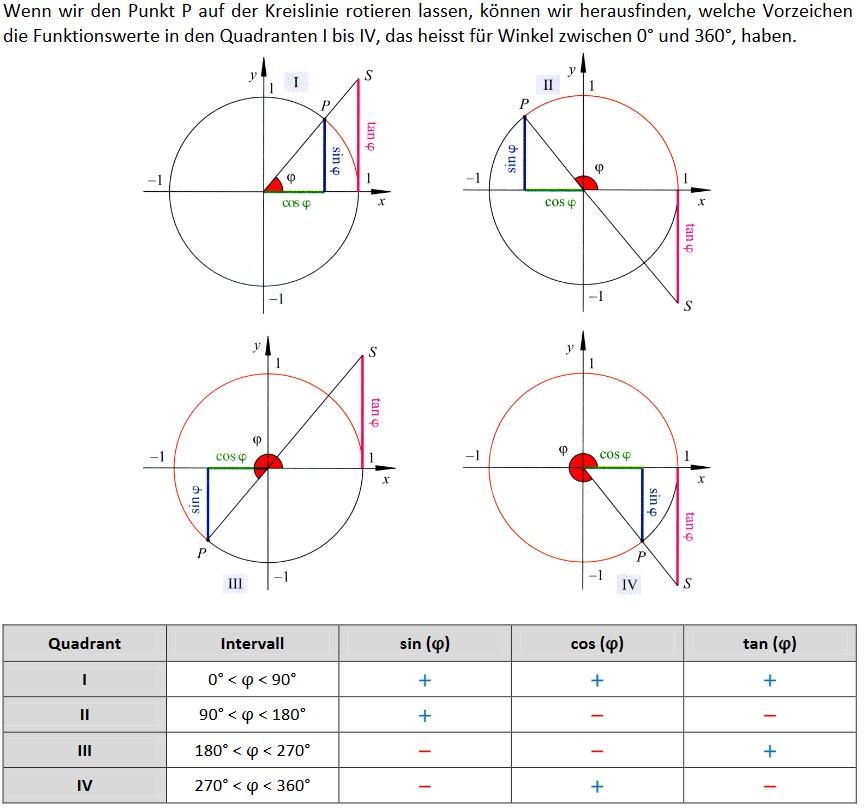
\includegraphics[scale=0.7]{einheitskreis4.PNG}

\subsection{Eigenschaften der Funktionen}
\begin{tabularx}{1\textwidth} {
    | >{\raggedright\arraybackslash}c
    | >{\raggedright\arraybackslash}X
    | >{\raggedright\arraybackslash}X
    | >{\raggedright\arraybackslash}X |}
  \hline
                              & \textbf{Sinus}                                                       & \textbf{Kosinus}                                                             & \textbf{Tangens}                                                                       \\\hline
  \textbf{Definitionsbereich} & $\left\{ x|x\in\mathbb{R}\right\}$ or $\left(-\infty,+\infty\right)$ & $\left\{ x|x\in\mathbb{R}\right\}$ or $\left(-\infty,+\infty\right)$         & $\mathbb{D}_f = \mathbb{R}\setminus\{\tfrac{\pi}{2} + k \cdot \pi, k \in \mathbb{Z}\}$ \\ \hline
  \textbf{Wertebereich}       & $\left[-1,1\right]$                                                  & $\left[-1,1\right]$                                                          & $\mathbb{W}_f = \mathbb{R}$                                                            \\ \hline
  \textbf{Periodizität}       & $2\pi$                                                               & $2\pi$                                                                       & $\pi$                                                                                  \\ \hline
  \textbf{Symmetrie}          & Punktsymetrisch zum Ursprung: Ungerade Funktion $\sin(-x)=-\sin(x)$  & Symetrisch zur y-Achse: gerade Funktion $\cos(x) = \cos(-x)$                 & Punktsymetrisch zum Ursprung: Ungerade Funktion $\tan(-x)=-\tan(x)$                    \\ \hline
  \textbf{Symmetrieachsen}    & $x=\frac{\pi}{2}+k\cdot \pi$ $k \in Z$                               & $x=k\cdot \pi$ $k \in Z$                                                     & $k \cdot \pi$                                                                          \\ \hline
  \textbf{Nullstellen}        & $x_k = k \cdot \pi$ $k \in \mathbb{Z}$                               & $x_k = \frac{\pi}{2} + k \cdot \pi$ $k \in \mathbb{Z}$    $k \in \mathbb{Z}$ & $x_k = k \cdot \pi$   $k \in \mathbb{Z}$                                               \\ \hline
  \textbf{Maxima}             & $x_k = \frac{\pi}{2} + k \cdot 2\pi$                                 & $x_k = k \cdot 2\pi$                                                         &                                                                                        \\ \hline
  \textbf{Minima}             & $x_k = \frac{3\pi}{2} + k \cdot 2\pi$                                & $x_k = \pi + k \cdot 2\pi$                                                   &                                                                                        \\ \hline
  \textbf{Es gilt}            & $\sin(x)=(\cos(x-\frac{\pi}{2})$)                                    & $\cos(x)=(\sin(x+\frac{\pi}{2})$)                                            & $\tan(x)=\frac{\sin(x)}{\cos(x)}$                                                      \\ \hline
\end{tabularx}

\newpage

\begin{multicols}{2}
  \subsection{Transformation der Sinusfunktion}
  \subsubsection{Allgemeine Sinusfunktion}
  Die allgemeine Sinusfunktion ist folgendermassen definiert:
  \[y=a\cdot\sin(b\cdot(x+u))+v\]
  \subsubsection{Strecken und Stauchen auf y-Achse}
  Parameter a: Strecken / Stauchen auf y-Achse (Amplitude): $y=a\cdot\sin(x)$ $a\in\mathbb{R}_{0}$

  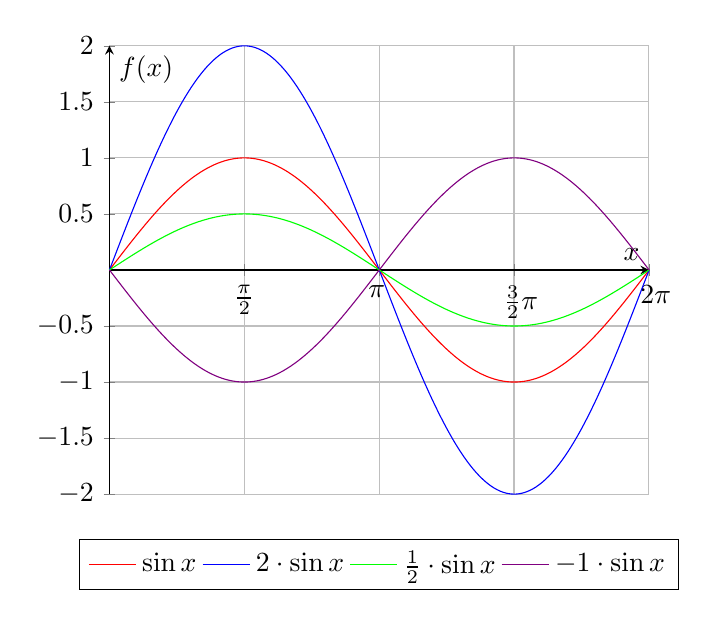
\begin{tikzpicture}
    \begin{axis}[
        clip=false,
        xmin=0,xmax=2*pi,
        xlabel= $x$,
        ylabel=$f(x)$,
        ymin=-2,ymax=2,
        ytick={-2,-1.5,-1,-0.5,0,0.5,1,1.5,2},
        axis lines=middle,
        grid,
        legend style={at={(0.5,-0.1)},
            anchor=north,legend columns=-1},
        %axis x line=middle,
        %axis y line=left,
        %     axis x line=middle,
        xtick={0,1.57,3.14,4.71,6.28},
        xticklabels={$0$, $\frac{\pi}{2}$,$\pi\,$,$\,\,\,\frac{3}{2}\pi$,$\,\,\,2\pi$},
        %xticklabel style={anchor=north west}
      ]
      \addplot[domain=0:2*pi,samples=200,red]{sin(deg(x))};
      \addlegendentry {$\sin x$};
      \addplot[domain=0:2*pi,samples=200,blue]{2*(sin(deg(x)))};
      \addlegendentry {$2\cdot \sin x$};
      \addplot[domain=0:2*pi,samples=200,green]{0.5*(sin(deg(x)))};
      \addlegendentry {$\frac{1}{2}\cdot \sin x$};
      \addplot[domain=0:2*pi,samples=200,violet]{-1*(sin(deg(x)))};
      \addlegendentry {$-1\cdot \sin x$};
    \end{axis}
  \end{tikzpicture}

  \begin{tabularx}{0.5\textwidth} {
      >{\centering\arraybackslash}c
      >{\centering\arraybackslash}c
      >{\centering\arraybackslash}c}
    \boldmath $|a|>1$ & \boldmath$0<|a|<1$ & \boldmath$|a|<0$      \\
    Streckung         & Stauchung          & Spiegelung an x-Achse \\
  \end{tabularx}

  \subsubsection{Strecken und Stauchen auf x-Achse}
  Parameter b: Strecken / Stauchen auf x-Achse: $y=sin(b\cdot x)$ $b\in\mathbb{R}^{+}$

  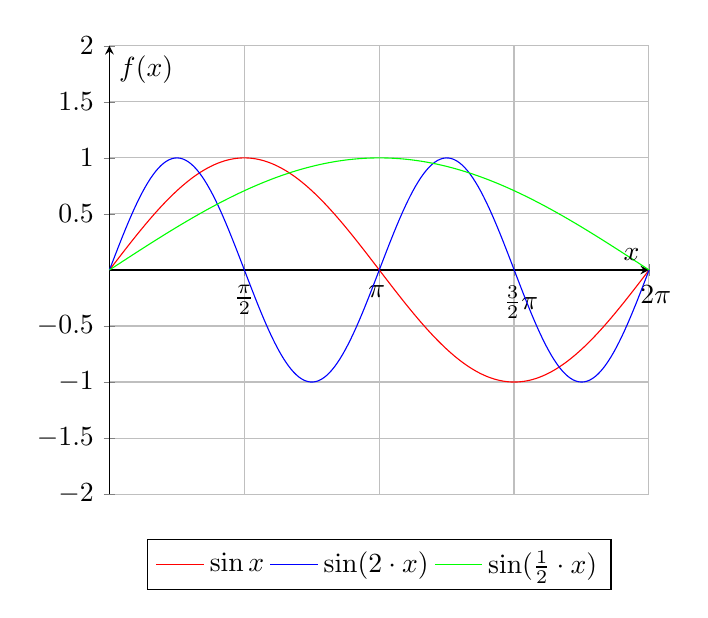
\begin{tikzpicture}
    \begin{axis}[
        clip=false,
        xmin=0,xmax=2*pi,
        xlabel= $x$,
        ylabel=$f(x)$,
        ymin=-2,ymax=2,
        ytick={-2,-1.5,-1,-0.5,0,0.5,1,1.5,2},
        axis lines=middle,
        grid,
        legend style={at={(0.5,-0.1)},
            anchor=north,legend columns=-1},
        %axis x line=middle,
        %axis y line=left,
        %     axis x line=middle,
        xtick={0,1.57,3.14,4.71,6.28},
        xticklabels={$0$, $\frac{\pi}{2}$,$\pi\,$,$\,\,\,\frac{3}{2}\pi$,$\,\,\,2\pi$},
        %xticklabel style={anchor=north west}
      ]
      \addplot[domain=0:2*pi,samples=200,red]{sin(deg(x))};
      \addlegendentry {$\sin x$};
      \addplot[domain=0:2*pi,samples=200,blue]{sin(deg(2*x))};
      \addlegendentry {$\sin(2\cdot x)$};
      \addplot[domain=0:2*pi,samples=200,green]{sin(deg(0.5*x))};
      \addlegendentry {$\sin(\frac{1}{2}\cdot x)$};


    \end{axis}
  \end{tikzpicture}

  \begin{tabularx}{0.5\textwidth} {
      >{\centering\arraybackslash}X
      >{\centering\arraybackslash}X}
    \boldmath $b>1$                     & \boldmath$0< b <1$                                                                        \\
    Stauchung in x-Richtung um den Faktor b.
    (kleinere Periode, höhere Frequenz) & Streckung in x-Richtung um den Faktor $\frac{1}{b}$.(grössere Periode, kleinere Frequenz) \\
  \end{tabularx}



  \subsubsection{Schieben in x-Richtung}
  Parameter u: Schieben in x-Richtung: $y=\sin(x+u)$ $u\in\mathbb{R}$

  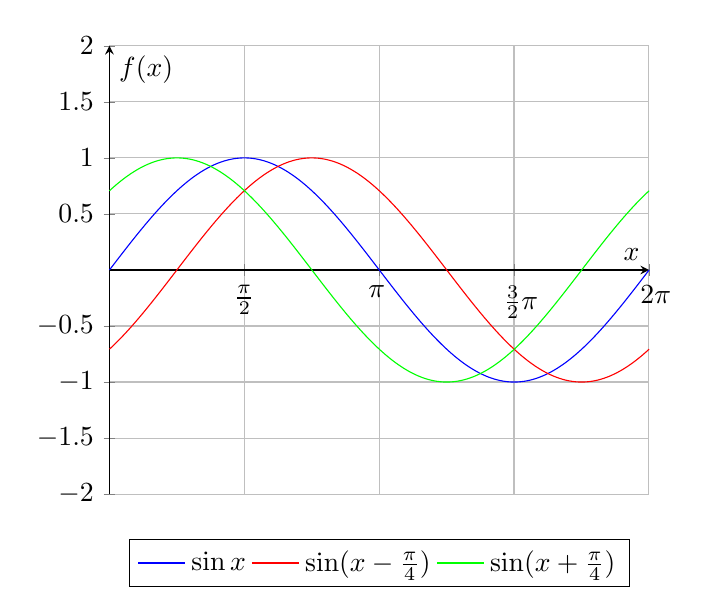
\begin{tikzpicture}
    \begin{axis}[
        clip=false,
        xmin=0,xmax=2*pi,
        xlabel= $x$,
        ylabel=$f(x)$,
        ymin=-2,ymax=2,
        ytick={-2,-1.5,-1,-0.5,0,0.5,1,1.5,2},
        axis lines=middle,
        grid,
        legend style={at={(0.5,-0.1)},
            anchor=north,legend columns=-1},
        %axis x line=middle,
        %axis y line=left,
        %     axis x line=middle,
        xtick={0,1.57,3.14,4.71,6.28},
        xticklabels={$0$, $\frac{\pi}{2}$,$\pi\,$,$\,\,\,\frac{3}{2}\pi$,$\,\,\,2\pi$},
        %xticklabel style={anchor=north west}
      ]
      \addplot[domain=0:2*pi,samples=200,blue]{sin(deg(x))};
      \addlegendentry {$\sin x$};
      \addplot[domain=0:2*pi,samples=200,red]{(sin(deg(x-0.785)))};
      \addlegendentry {$\sin (x-\frac{\pi}{4})$};
      \addplot[domain=0:2*pi,samples=200,green]{(sin(deg(x+0.785)))};
      \addlegendentry {$\sin (x+\frac{\pi}{4})$};

    \end{axis}
  \end{tikzpicture}

  \begin{tabularx}{0.5\textwidth} {
      >{\centering\arraybackslash}X
      >{\centering\arraybackslash}X}
    \boldmath $u>1$          & \boldmath$u < 0$          \\
    Verschiebung nach links. & Verschiebung nach rechts. \\
  \end{tabularx}



  \subsubsection{Schieben in y-Richtung}
  Parameter v: Schieben in y-Richtung:  $y=a\cdot\sin(x)+v$ $v\in\mathbb{R}$

  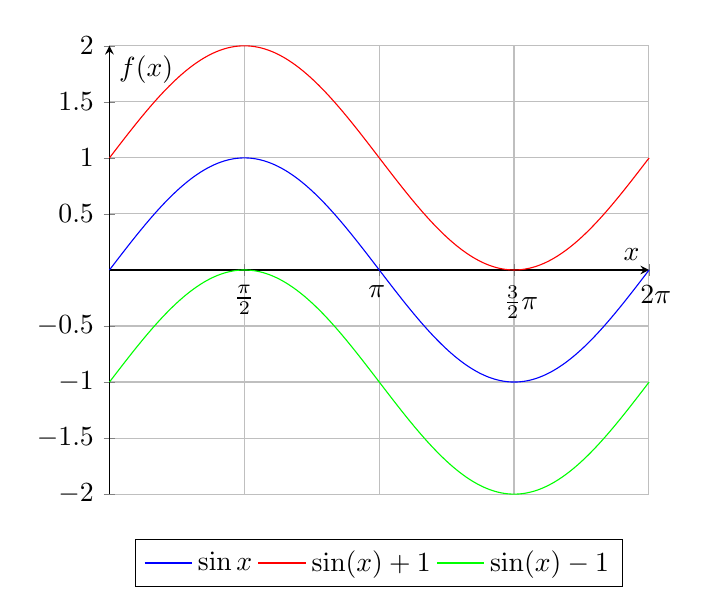
\begin{tikzpicture}
    \begin{axis}[
        clip=false,
        xmin=0,xmax=2*pi,
        xlabel= $x$,
        ylabel=$f(x)$,
        ymin=-2,ymax=2,
        ytick={-2,-1.5,-1,-0.5,0,0.5,1,1.5,2},
        axis lines=middle,
        grid,
        legend style={at={(0.5,-0.1)},
            anchor=north,legend columns=-1},
        %axis x line=middle,
        %axis y line=left,
        %     axis x line=middle,
        xtick={0,1.57,3.14,4.71,6.28},
        xticklabels={$0$, $\frac{\pi}{2}$,$\pi\,$,$\,\,\,\frac{3}{2}\pi$,$\,\,\,2\pi$},
        %xticklabel style={anchor=north west}
      ]
      \addplot[domain=0:2*pi,samples=200,blue]{sin(deg(x))};
      \addlegendentry {$\sin x$};
      \addplot[domain=0:2*pi,samples=200,red]{(sin(deg(x))+1)};
      \addlegendentry {$\sin (x)+1$};
      \addplot[domain=0:2*pi,samples=200,green]{(sin(deg(x))-1)};
      \addlegendentry {$\sin (x)-1$};

    \end{axis}
  \end{tikzpicture}

  \begin{tabularx}{0.5\textwidth} {
      >{\centering\arraybackslash}X
      >{\centering\arraybackslash}X}
    \boldmath $v >1$        & \boldmath$v < 0$         \\
    Verschiebung nach oben. & Verschiebung nach unten. \\
  \end{tabularx}

\end{multicols}
\newpage{}





\newpage{}
\section{Goniometrie}
\subsubsection{Identitäten}
\begin{multicols}{2}

  \textbf{Kofunktionen}
  \begin{align*}
     & \sin(\frac{\pi}{2} - x) & = \cos x \\
     & \cos(\frac{\pi}{2} - x) & = \sin x \\
     & \tan(\frac{\pi}{2} - x) & = \cot x \\
     & \cot(\frac{\pi}{2} - x) & = \tan x \\
     & \sec(\frac{\pi}{2} - x) & = \csc x \\
     & \csc(\frac{\pi}{2} - x) & = \sec x
  \end{align*}

  \textbf{Symmetrie}
  \begin{align*}
    \sin(-x) & = - \sin x \\
    \cos(-x) & = \cos x   \\
    \tan(-x) & = -\tan x
  \end{align*}

  \textbf{Doppelter Winkel}
  \begin{align*}
    \sin(2x) & = 2 \sin x \cos x               \\
    \cos(2x) & = \cos^2 x - \sin^2 x           \\
             & = 2 \cos^2 x - 1                \\
             & = 1 - 2 \sin^2 x                \\
    \tan(2x) & = \frac{2 \tan x}{1 - \tan^2 x}
  \end{align*}

  \textbf{Halber Winkel}
  \begin{align*}
    \sin \frac{x}{2} & = \pm \sqrt{ \frac{1 - \cos x }{2} } \\
    \cos \frac{x}{2} & = \pm \sqrt{ \frac{1 + \cos x }{2} } \\
    \tan \frac{x}{2} & = \frac{1 - \cos x }{\sin x}         \\
                     & = \frac{ \sin x }{ 1 + \cos x }
  \end{align*}

  \textbf{Exponent Reduktion}
  \begin{align*}
    \sin^2 x & = \frac{1 - \cos 2x}{2}               \\
    \sin^4x  & = (\frac{1 - \cos 2x}{2})^2           \\
    \cos^2 x & = \frac{1 + \cos 2x}{2}               \\
    \cos^4x  & = (\frac{1 + \cos 2x}{2})^2           \\
    \tan^2 x & = \frac{1 - \cos 2x}{1 + \cos 2x}     \\
    \tan^4 x & =( \frac{1 - \cos 2x}{1 + \cos 2x})^2
  \end{align*}

  \textbf{Pythagoras}
  \begin{align*}
    \sin^2 x + \cos^2 x & = 1        \\
    1 + \tan^2 x        & = \sec^2 x \\
    1 + \cot^2 x        & = \csc^2 x
  \end{align*}

  \textbf{Umkehrwert}
  \begin{align*}
    \cot x & = \frac{1}{\tan x} \\
    \csc x & = \frac{1}{\sin x} \\
    \sec x & = \frac{1}{\cos x}
  \end{align*}

  \textbf{Summe und Differenz von Winkel}
  \begin{align*}
    \sin(x + y) & = \sin x \cos y + \cos x \sin y             \\
    \sin(x - y) & = \sin x \cos y - \cos x \sin y             \\
    \cos(x + y) & = \cos x \cos y - \sin x \sin y             \\
    \cos(x - y) & = \cos x \cos y + \sin x \sin y             \\
    \tan(x + y) & = \frac{\tan x + \tan y}{1 - \tan x \tan y} \\
    \tan(x - y) & = \frac{\tan x - \tan y}{1 + \tan x \tan y}
  \end{align*}

  \textbf{Produkt zu Summe}
  \begin{align*}
    \sin x \sin y & = \frac{1}{2}\big[\cos(x - y) - \cos(x + y)\big] \\
    \cos x \cos y & = \frac{1}{2}\big[\cos(x - y) + \cos(x + y)\big] \\
    \sin x \cos y & = \frac{1}{2}\big[\sin(x + y) + \sin(x - y)\big] \\
    \tan x \tan y & = \frac{ \tan x + \tan y }{ \cot x + \cot y }    \\
    \tan x \cot y & = \frac{ \tan x + \cot y }{ \cot x + \tan y }
  \end{align*}

  \textbf{Summe Zu Produkt}
  \begin{align*}
    \sin x + \sin y & = 2 \sin \Big( \frac{x + y}{2} \Big) \cos \Big( \frac{x - y}{2} \Big)  \\
    \sin x - \sin y & = 2 \cos \Big( \frac{x + y}{2} \Big) \sin \Big( \frac{x - y}{2} \Big)  \\
    \cos x + \cos y & = 2 \cos \Big( \frac{x + y}{2} \Big) \cos \Big( \frac{x - y}{2} \Big)  \\
    \cos x - \cos y & = -2 \sin \Big( \frac{x + y}{2} \Big) \sin \Big( \frac{x - y}{2} \Big) \\
    \tan x + \tan y & = \frac{ \sin(x + y) }{ \cos x \cos y}                                 \\
    \tan x - \tan y & = \frac{ \sin(x - y) }{ \cos x \cos y}                                 \\
  \end{align*}

\end{multicols}
\newpage
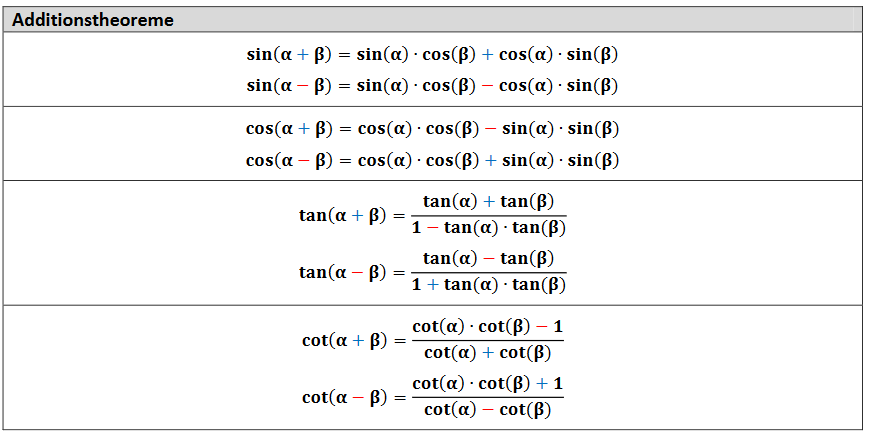
\includegraphics[scale=0.7]{gon2.PNG}

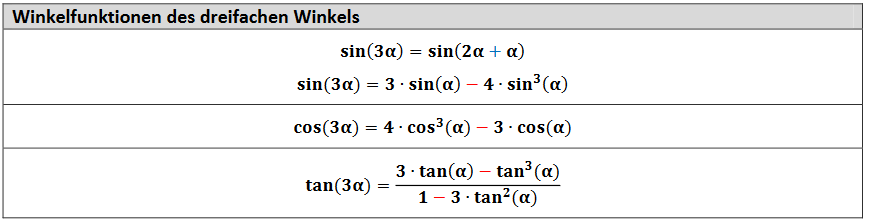
\includegraphics[scale=0.7]{gon4.PNG}

\newpage


\end{document}
